% This LaTeX document needs to be compiled with XeLaTeX.
%!mode::"TeX:UTF-8"
% !TEX program = xelatex
\documentclass[
  10
]{article}
\usepackage[margin=2cm,includehead=true,includefoot=true,centering,]{geometry}
\usepackage{xcolor}
\usepackage{listings}
\usepackage{ucharclasses}
\usepackage{hyperref}
\usepackage{amsmath,amssymb}
\usepackage{amsfonts}
\usepackage[version=4]{mhchem}
\usepackage{polyglossia}
\usepackage{fontspec}
\usepackage[fontset=none]{ctex}
\usepackage[export]{adjustbox}
\usepackage{tabularx}
\usepackage{booktabs}

\usepackage{setspace}
\setstretch{1.2}

\makeatletter
\@ifundefined{KOMAClassName}{% if non-KOMA class
  \IfFileExists{parskip.sty}{%
    \usepackage{parskip}
  }{% else
    \setlength{\parindent}{0pt}
    \setlength{\parskip}{6pt plus 2pt minus 1pt}}
}{% if KOMA class
  \KOMAoptions{parskip=half}}
\makeatother
\usepackage{longtable,booktabs,array}
\newcounter{none} % for unnumbered tables
\usepackage{calc} % for calculating minipage widths
% Correct order of tables after \paragraph or \subparagraph
\usepackage{etoolbox}
\makeatletter
\patchcmd\longtable{\par}{\if@noskipsec\mbox{}\fi\par}{}{}
\makeatother
% Allow footnotes in longtable head/foot
\IfFileExists{footnotehyper.sty}{\usepackage{footnotehyper}}{\usepackage{footnote}}
\makesavenoteenv{longtable}
\setlength{\emergencystretch}{3em} % prevent overfull lines
\providecommand{\tightlist}{%
  \setlength{\itemsep}{0pt}\setlength{\parskip}{0pt}}

\hypersetup{colorlinks=true, linkcolor=blue, filecolor=magenta, urlcolor=cyan,}
\urlstyle{same}

% 代码高亮设置
\usepackage{xcolor}
\definecolor{codegreen}{rgb}{0,0.6,0}
\definecolor{codegray}{rgb}{0.5,0.5,0.5}
\definecolor{codepurple}{rgb}{0.58,0,0.82}
\definecolor{backcolour}{rgb}{0.95,0.95,0.92}

\lstset{
    backgroundcolor=\color{backcolour},
    commentstyle=\color{codegreen},
    keywordstyle=\color{magenta},
    numberstyle=\tiny\color{codegray},
    stringstyle=\color{codepurple},
    basicstyle=\ttfamily\footnotesize,
    breakatwhitespace=false,
    breaklines=true,
    captionpos=b,
    keepspaces=true,
    numbers=left,
    numbersep=5pt,
    showspaces=false,
    showstringspaces=false,
    showtabs=false,
    tabsize=4,
    frame=single,
    framerule=0pt,
}

% 中文图表前缀
\usepackage{caption}
\captionsetup{labelfont=bf,labelsep=space}
\renewcommand{\tablename}{表}
\renewcommand{\figurename}{图}

\usepackage{colortbl}
\definecolor{table-row-color}{HTML}{999999}
\definecolor{table-rule-color}{HTML}{999999}
%\arrayrulecolor{black!40}
\arrayrulecolor{table-rule-color}     % color of \toprule, \midrule, \bottomrule
\setlength{\aboverulesep}{0pt}
\setlength{\belowrulesep}{0pt}

\setotherlanguages{english}
\IfFontExistsTF{Times New Roman}
{\setmainfont{Times New Roman}}
{\IfFontExistsTF{Times}
  {\setmainfont{Times}}
  {\IfFontExistsTF{Liberation Serif}
    {\setmainfont{Liberation Serif}}
    {\setmainfont{Times New Roman}}
}}
\newcommand*{\CJKMainFontName}{Songti SC Regular}
\IfFontExistsTF{Songti SC Regular}{}{%
  \IfFontExistsTF{Songti SC}{\renewcommand*{\CJKMainFontName}{Songti SC}}{%
    \IfFontExistsTF{STSongti-SC-Regular}{\renewcommand*{\CJKMainFontName}{STSongti-SC-Regular}}{%
      \IfFontExistsTF{STSong}{\renewcommand*{\CJKMainFontName}{STSong}}{%
        \IfFontExistsTF{FandolSong-Regular}{\renewcommand*{\CJKMainFontName}{FandolSong-Regular}}{}%
      }%
    }%
  }%
}
\setCJKmainfont{\CJKMainFontName}
\setCJKmonofont{\CJKMainFontName}
\newcommand*{\CJKSansFontName}{Heiti SC Light}
\IfFontExistsTF{Heiti SC Light}{}{%
  \IfFontExistsTF{STHeitiSC-Light}{\renewcommand*{\CJKSansFontName}{STHeitiSC-Light}}{%
    \IfFontExistsTF{STHeiti Light}{\renewcommand*{\CJKSansFontName}{STHeiti Light}}{%
      \IfFontExistsTF{Heiti SC}{\renewcommand*{\CJKSansFontName}{Heiti SC}}{%
        \IfFontExistsTF{STHeiti}{\renewcommand*{\CJKSansFontName}{STHeiti}}{%
          \IfFontExistsTF{FandolHei-Regular}{\renewcommand*{\CJKSansFontName}{FandolHei-Regular}}{}%
        }%
      }%
    }%
  }%
}
\setCJKsansfont{\CJKSansFontName}
\setCJKfamilyfont{hei}{\CJKSansFontName}
\setCJKfamilyfont{song}{\CJKMainFontName}
\providecommand{\heiti}{\CJKfamily{hei}}

\author{}
\date{}

\begin{document}

\section*{第3章\quad 人工智能基础}
\subsection*{3.1\quad 人工智能概述}

\begin{figure}[htbp]
\centering
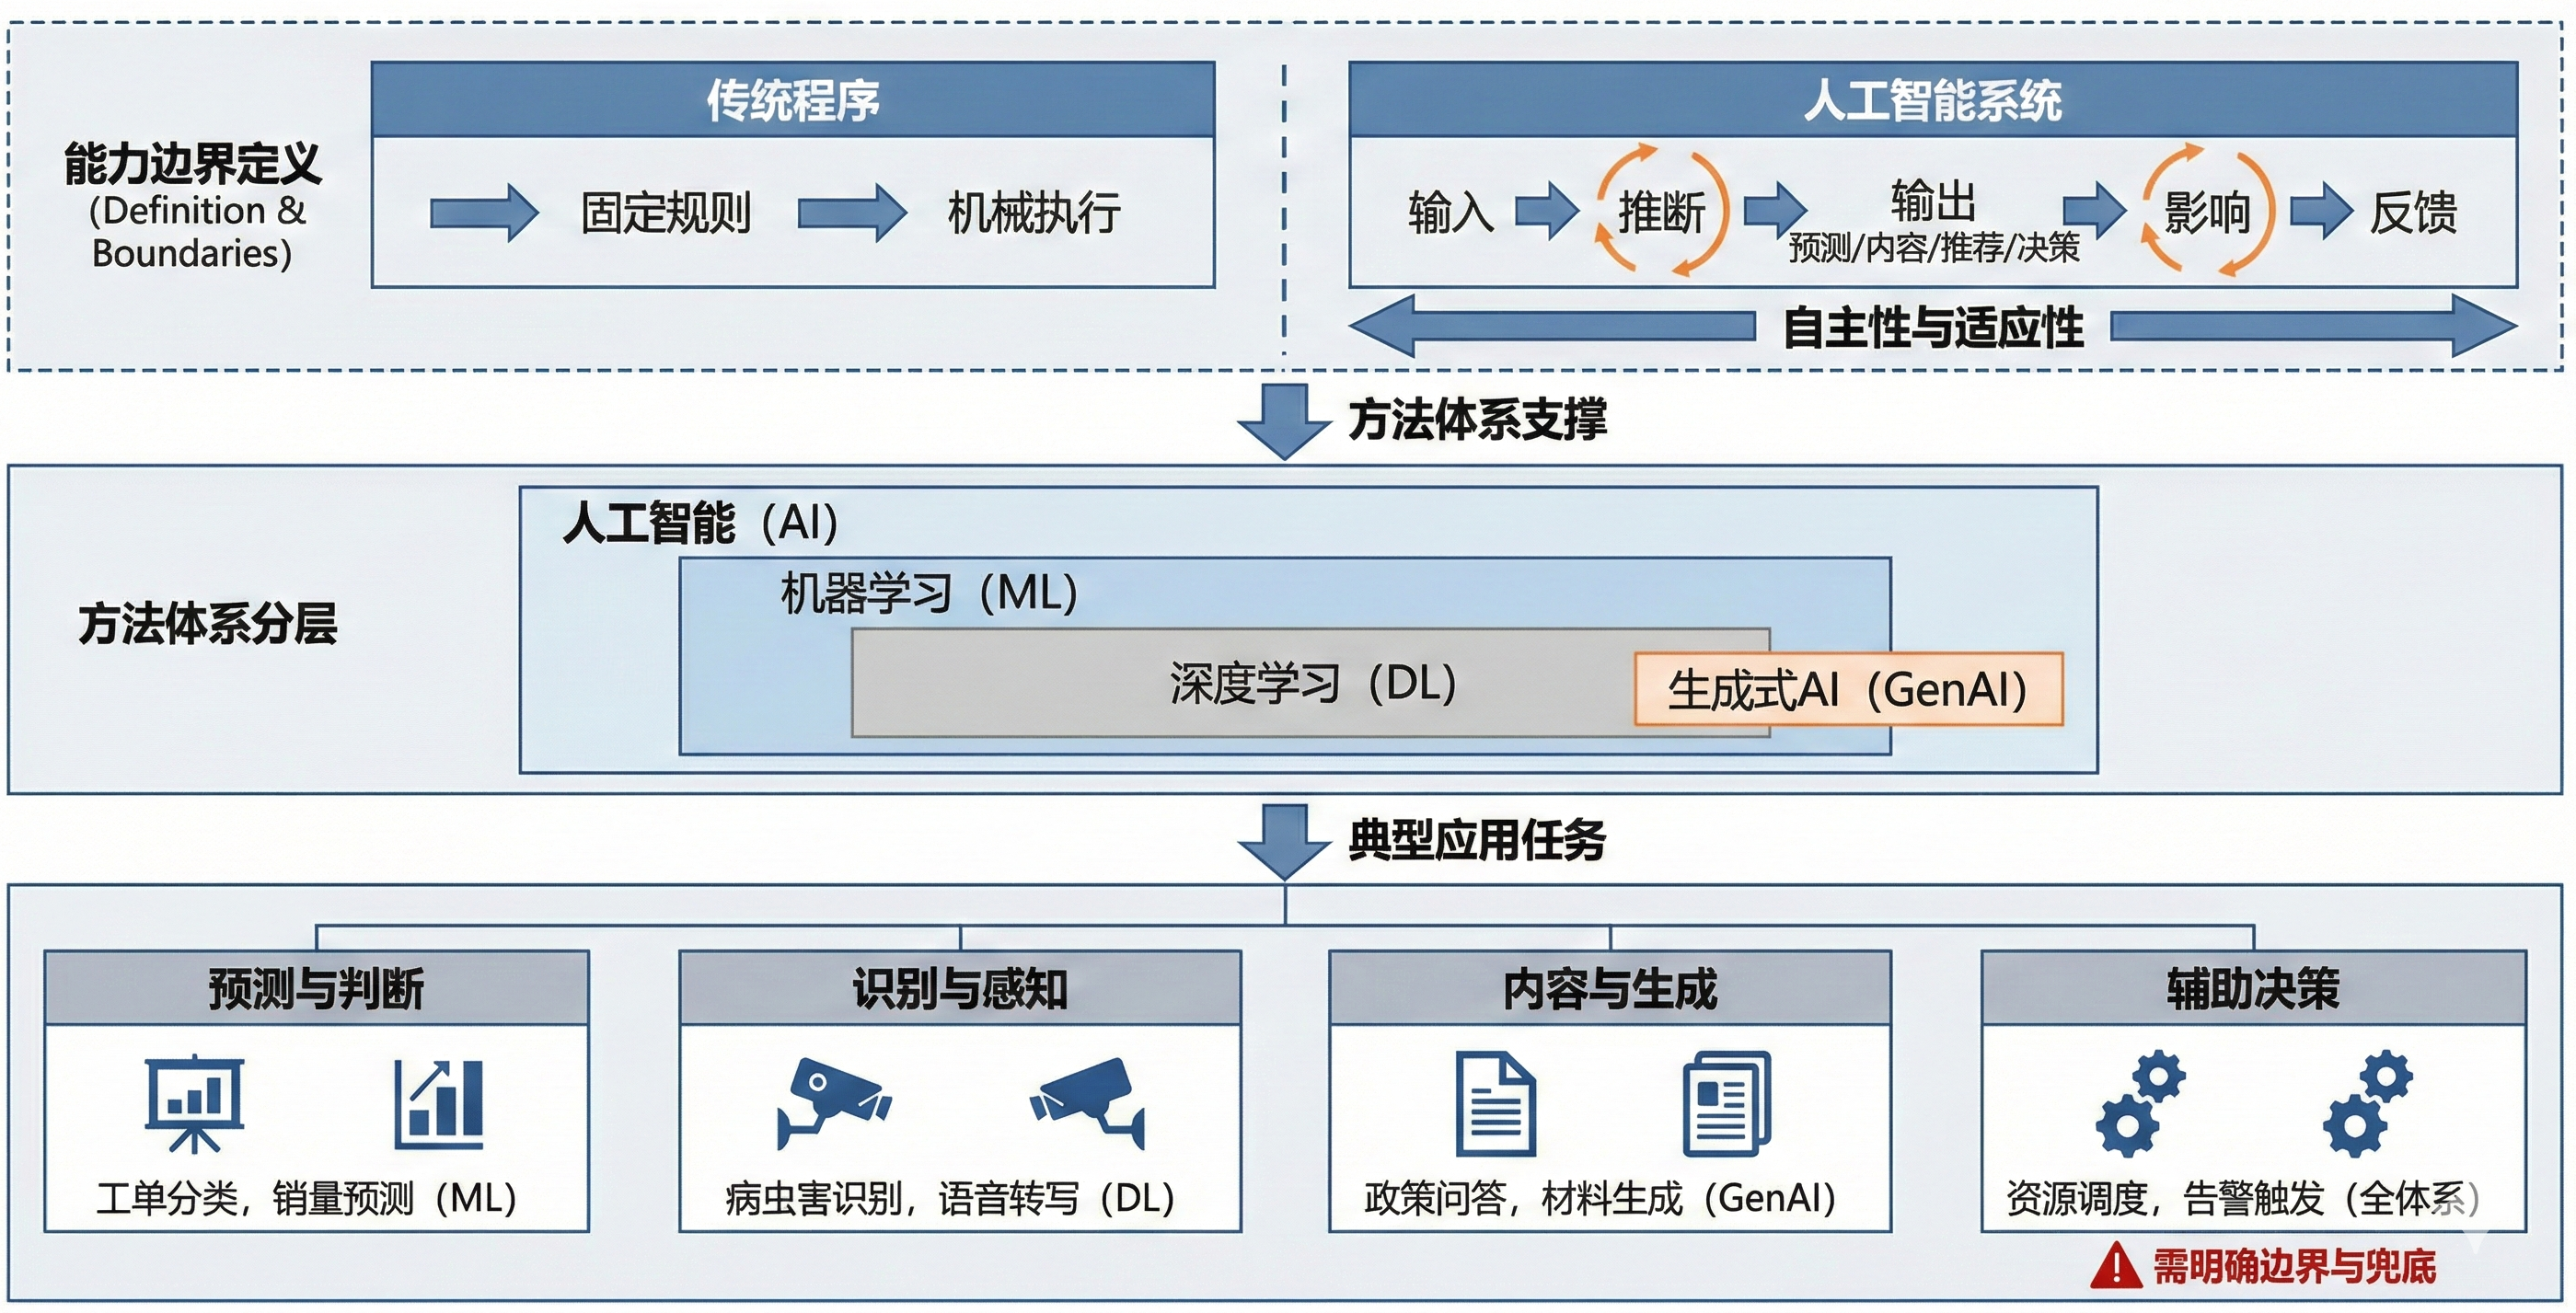
\includegraphics[width=0.9\textwidth]{figures/fig-ai-ml-dl-genai}
\caption{人工智能概念体系总览。}
\label{fig:ai-ml-dl-genai}
\end{figure}

\subsubsection*{3.1.1\quad 人工智能定义}
\noindent 人工智能是可工程化落地的系统,不是单一模型或单一功能。系统围绕明确或隐含的目标运行,从其接收的输入中进行推断,生成预测、内容、推荐或决策等输出,并且这些输出能够影响物理或虚拟环境。不同系统在自主性水平以及部署后的适应性方面存在差异。这样的表述强调目标、推断、输出、影响、自主与适应这一条可核对、可审计的链条,便于在跨学科沟通与项目交付中保持一致。

\noindent 这里所说的机器系统,并不等同于机器人设备,而是指能够被工程化实现并在一定规则与约束下运行的系统形态。它可能是纯软件系统,如热线工单分派、政策问答与材料清单生成,也可能是软硬一体的系统,如带摄像头的分拣设备、巡检终端或无人机采集与识别系统。之所以强调系统,是因为人工智能落地的成败通常不取决于某个模型的单点表现,而取决于数据来源与口径、流程嵌入方式、权限边界、人工复核与上线监控等要素是否形成闭环。这些要素共同决定系统输出能否稳定地支持业务动作。

\noindent 目标需要被明确区分为显式与隐含两类。显式目标是写入需求说明或指标体系的目标,如将工单按类别准确分派、降低备货浪费、缩短平均响应时长。隐含目标则是系统在运行中可能默认追求的方向,如尽可能提高点击率或响应速度。目标并非中性技术参数,它会直接牵引数据收集、模型优化方向与业务风险边界。同一套数据与技术在不同目标约束下可能导向完全不同的行为结果。因此目标的设定与约束首先是治理与管理问题,其次才是技术实现问题。

\noindent 从输入中进行推断是区分人工智能系统与一般自动化的关键。推断意味着系统不是机械复制输入或执行固定模板,而是基于规则、知识或数据训练得到的模型,对输入进行处理并形成对输出的判断。换言之,系统能够在一定范围内把既有经验迁移到新样本、新情形上,给出可重复、可检验的输出。反过来,如果某个流程仅是固定规则的机械串联,无推断机制,也不具备对新情况的处理能力,那么更适合被称为流程自动化,而不宜泛化称作人工智能。这种边界澄清的目的不是抬高门槛,而是为后续方法选择、效果评估与责任划分提供共同语言。

\noindent 在输出层面,将预测、内容、推荐、决策四类输出写清楚,可以把抽象能力直接对齐到业务动作。预测对应对未来或未知量的估计,如客流、销量、价格、病害风险。内容对应表达性输出,如宣讲稿、摘要、海报文案、材料清单整理。推荐对应候选项的排序或匹配,如政策匹配、课程推荐、资源配置建议。决策则对应触发动作或给出选择,如是否告警、是否进入人工复核、是否进入加急流程。只要输出能够影响物理或虚拟环境,就必须进一步讨论责任、边界与可追溯性。输出如何进入业务流程、由谁确认、如何留痕、如何纠错,决定了系统是辅助还是替代,也决定了风险控制的最低配置。

\noindent 最后,自主性与部署后的适应性用于刻画系统运行方式与风险管理强度。自主性越高,系统越可能在较少人工介入下连续运行。适应性越强,系统越可能在上线后根据新数据或新交互调整行为。一般而言,这两项能力越强,潜在效率收益越大,但对监控、审计、权限控制、阈值策略与兜底机制的要求也越高,且需要更明确地界定系统输出的可用范围与人应当介入的触发条件。

\noindent 放在乡村经营语境中,可以用一个最小案例把上述链条落到业务上。以政务热线工单分派为例,系统接收群众留言、地点与历史工单信息,通过推断识别问题类别与紧急程度,输出分派部门与响应时限,并据此影响工单流转、人员调度与现场处置。这个过程之所以可被称为人工智能系统,不在于它是否使用了复杂模型,而在于它围绕目标形成了从输入到输出的推断机制,并且输出被嵌入到可追溯、可纠错的业务流程之中。

\subsubsection*{3.1.2\quad 人工智能、机器学习、深度学习与生成式AI的区别}
\begin{figure}[htbp]
\centering
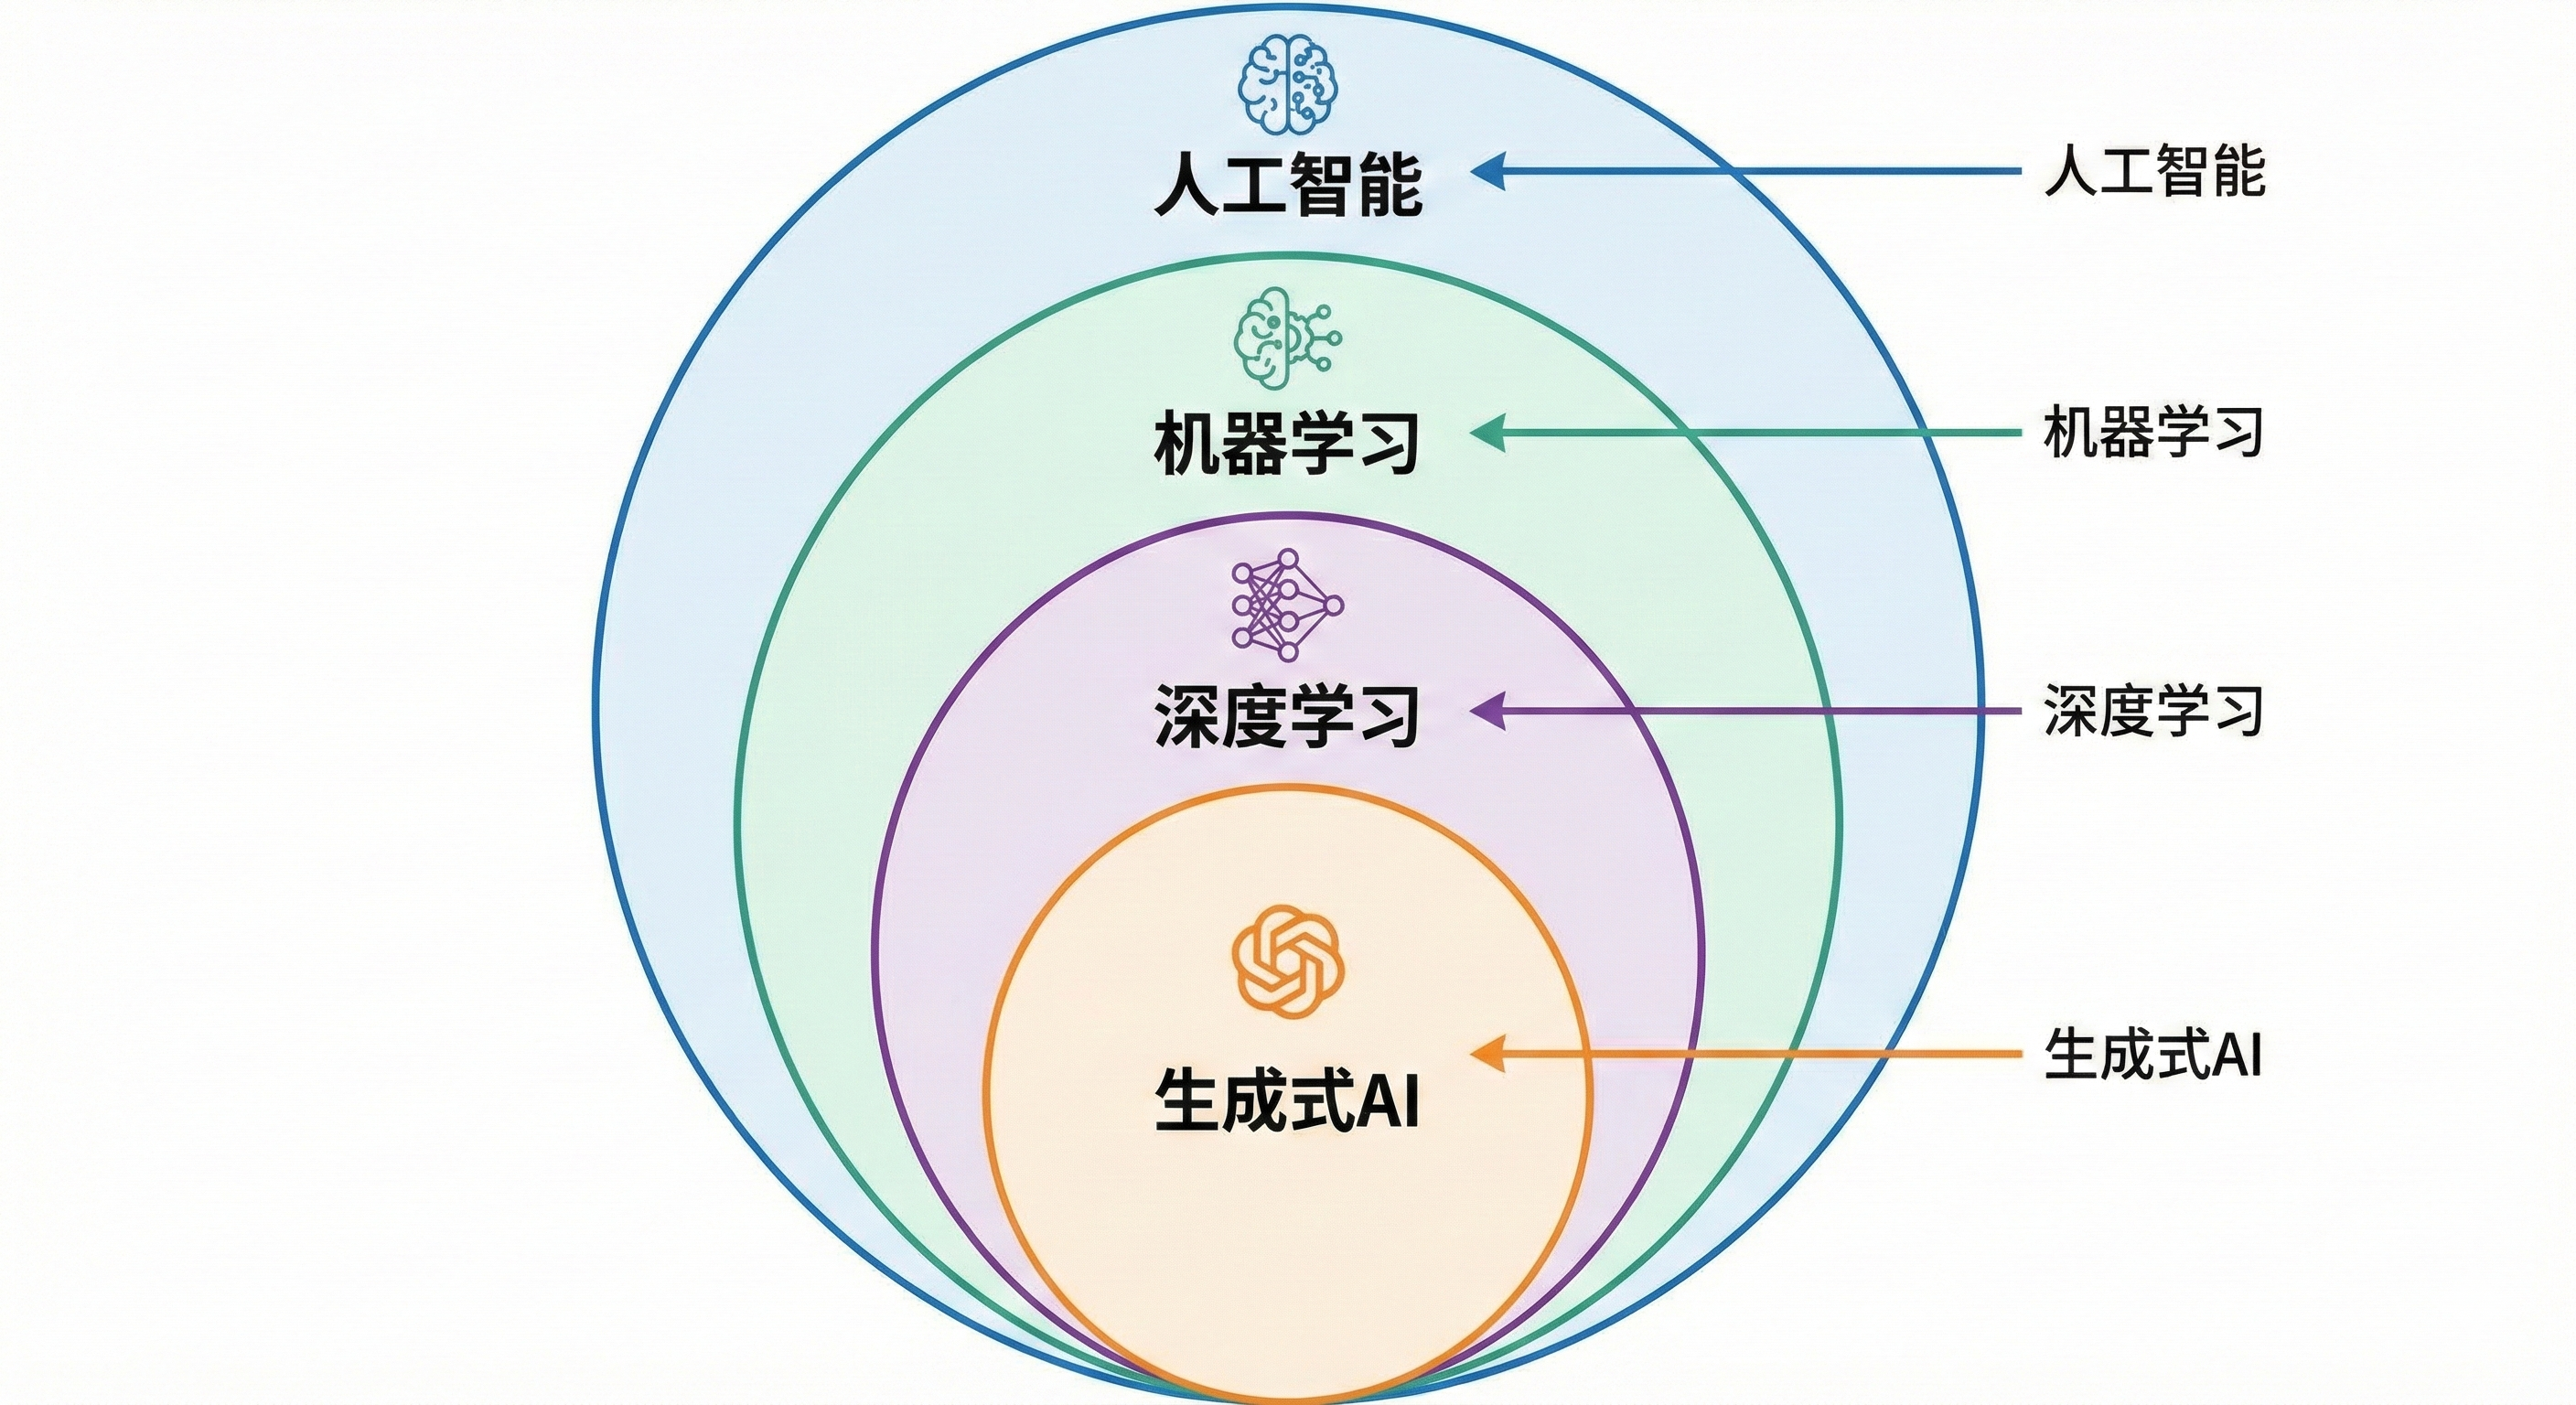
\includegraphics[width=0.9\textwidth]{figures/fig-ai-concept-hierarchy}
\caption{人工智能、机器学习、深度学习与生成式AI的概念层级与区别。}
\label{fig:ai-concept-hierarchy}
\end{figure}

\noindent 人工智能是总称,关注的是机器系统是否以目标为导向,能够基于输入进行推断并产生输出,且该输出能够影响物理或虚拟环境。系统之间在自主性与部署后适应性方面存在差异。这里强调系统,意味着人工智能并非等同于某个模型或某段代码,而是由数据、规则或模型、流程、权限、人工复核与监控等要素共同构成的业务机制。因而在乡村经营中,许多高价值的智能化并不依赖复杂模型,例如通过规则与流程实现的工单分派、资格初筛、风险分级,只要其输出是围绕明确目标形成的、可重复使用并能在一定范围内泛化到新情况的推断结果,就属于人工智能系统在业务链条中的一种实现方式。

\noindent 机器学习是人工智能的一条重要实现路径,其核心在于从数据中学习可泛化的映射关系。工程上,机器学习用训练数据把输入与输出之间的关系固化为模型,使系统能够在未见样本上进行预测或判断。管理上,它意味着用数据与统计规律替代部分人工经验与手写规则,从而在不确定环境中输出概率性或统计意义上的结论。机器学习尤其适合乡村经营中大量结构化数据场景,如台账与交易记录、客流与销量序列、工单与满意度指标等,因为这些数据容易形成稳定的字段口径、明确的评价指标与可持续迭代的反馈闭环。

\noindent 深度学习是机器学习的子集,其典型优势来自多层表示学习。系统能够在训练中自动学习从低层特征到高层语义的表示,降低对人工特征设计的依赖。这使其在图像、语音、文本等非结构化数据上更具竞争力,但也通常意味着更高的数据规模要求、更显著的标注与训练工程成本,以及更强的算力与运维能力约束。对乡村场景而言,凡是输入以图片、语音或长文本为主且模式复杂的任务,深度学习更常见,例如病虫害识别、分级分拣与遥感解译,访谈语音转写与结构化归档,以及长政策文本的要点抽取与归纳等。

\noindent 面对不同任务应结合目标、数据与流程约束选择相应的人工智能方法,确保效果、成本与风险可控。当目标是预测或判断,且数据主要呈现为表格台账与结构化字段时,优先采用机器学习,通常成本更可控、评估更清晰、上线更稳定。当输入以图片、语音或长文本为主且任务复杂、传统特征工程难以奏效时,再考虑深度学习,并在立项阶段同步评估标注成本、算力资源与运维能力。当目标是表达、整理、生成或对话,并且业务流程能够容纳引用约束与人工核验时,才考虑生成式AI,并将核验与权限边界作为交付验收项。至于系统输出直接触发资源分配、资金发放、执法处置等自动决策型应用,应在目标定义、权限控制、审计记录、风险阈值与兜底机制明确之后再推进,避免把模型判断或生成内容直接等同为可追责决策。

\subsubsection*{3.1.3\quad 人工智能与传统程序}
\noindent 传统程序把业务规则写进代码里,系统按既定流程执行。学习型系统把一部分规则交给数据与训练过程,让模型从样本中学出规律,再对新输入做出推断。这种差异决定了两类系统在建设方式、评估方式与风险控制上都不一样。

\noindent 传统程序要改得更好,通常是补规则、改代码、加校验,再通过测试上线。学习型系统要改得更好,通常要先把数据口径和标注方式理顺,再训练、评估、上线观测并持续迭代。它的输出往往带有概率性,需要用指标、阈值、人工复核与留痕来保证可用。

\noindent 规则清晰、责任边界要求严格、变化不大的流程更适合传统程序,例如资格条件明确的审核初筛、台账字段校验与流程提醒。规则难穷举、输入复杂或变化快的任务更适合学习型方法,例如工单分派中的类别识别、图片中的病虫害识别、长文本中的要点抽取与归纳。

\noindent 选型时可以先问一个问题,关键规则能不能写清楚并覆盖大多数情况。能写清楚且长期稳定就优先采用规则与流程自动化,写不清楚或需要从大量历史数据里找规律就考虑机器学习或深度学习。

\noindent 学习型系统也会带来新的代价,包括数据采集与标注成本、训练与运维成本、解释性与稳定性下降的风险。项目评审除了看效果,还要看数据来源是否可靠、指标是否可监控、上线后是否能持续维护与纠偏。

\begin{table}[h]
\centering
\caption{学习型系统与传统程序的对照}
\begin{tabular}{@{}llllll@{}}
\toprule
知识来源 & 开发方式 & 改进方式 & 适用输入 & 可解释性 & 部署维护 \\ \midrule
规则与流程 & 编写规则 & 改规则和改代码 & 结构化为主 & 高 & 相对稳定 \\
数据与训练 & 训练模型 & 数据和训练迭代 & 复杂与非结构化 & 中等或较低 & 需持续监测 \\ \bottomrule
\end{tabular}
\end{table}

\subsection*{3.2\quad 人工智能发展简史}
\subsubsection*{3.2.1\quad 符号推理与专家系统}
\subsubsection*{3.2.2\quad 统计学习与数据驱动方法}
\subsubsection*{3.2.3\quad 深度学习兴起}
\subsubsection*{3.2.4\quad 生成式模型与大规模模型概览}

\subsection*{3.3\quad 机器学习基础}
\subsubsection*{3.3.1\quad 关键对象与术语}
\noindent \textbf{一\quad 任务 数据与样本\quad 基本对象与形式化表示}

\noindent 机器学习研究的直接对象是学习问题的形式化表达,而不是孤立的算法技巧。一个学习系统要成立,首先必须明确三件事。系统要完成的任务是什么,系统将从何种经验中改进,以及用何种性能度量来判定改进是否发生。任务给出输出的语义与形式,经验规定可用于学习的信息来源,性能度量则决定训练与比较模型时好坏的标尺。三者共同构成学习问题的边界条件。边界不清,训练过程即便收敛,也可能是在优化与真实目标不一致的替代目标。

\noindent 在形式化层面,最常用的表达是区分输入与输出。通常用 $X$ 表示输入数据,常见形式是特征矩阵或设计矩阵,用 $y$ 表示输出数据,也就是目标、标签或响应。$X$ 表示预测时可获得的描述信息,$y$ 表示训练阶段用作监督信号而在预测时不可直接使用的目标信息。以房价预测为例,$X$ 可以包含面积、户型、地段、楼龄、周边配套等属性,$y$ 是成交价格。训练阶段模型观察 $(X, y)$ 来学习映射规律。部署阶段模型仅接收新的 $X$,输出预测值 $\hat{y}$。这一区分看似只是符号约定,实质上规定了信息可得性的硬约束。任何预测时无法获得的信息,都不应被纳入 $X$。如果把未来信息或与目标几乎同义的字段混入特征,离线指标往往会异常乐观,而上线表现会迅速变差。

\noindent 在 $X$ 与 $y$ 的表示下,数据集由大量样本组成。样本是学习与评估的基本单位,通常对应 $X$ 的一行,也就是一个输入实例的特征向量。特征对应 $X$ 的一列,表示对所有样本以同一规则测量或抽取的属性。仍以房价为例,每套房子是一条样本,面积、卧室数、是否学区房是不同特征。将数据组织为矩阵并非为了形式美观,而是为了把异质对象统一成可计算的表示,从而使学习一个从 $X$ 到 $y$ 的映射成为明确的数学问题。

\noindent 监督学习中的标签应被视为一种观测结果,而不是天然真值。很多任务的标签来自人工标注、业务规则或延迟反馈,因此不可避免地包含噪声、口径不一致以及随时间变化的漂移。以垃圾信息识别为例,$X$ 可由邮件正文、标题、发件域名、历史交互等构成,$y$ 为垃圾或非垃圾。对于边界邮件,不同标注者或不同时期的策略可能给出不同结论。这类不一致会直接体现在模型可达到的上限与误差形态之中。因此,标签定义的清晰性、稳定性与可复现性,是模型性能与实验可信度的前置条件,而不是训练之后才考虑的附属问题。

\noindent 训练与评估的分离是学习问题成立的基本要求。用同一批数据既训练又评估,会把对已见样本的拟合误当作对未见样本的能力,从而得到系统性偏高的结论。实践中通常将数据划分为训练集、验证集与测试集。训练集用于拟合模型参数,验证集用于模型选择与超参数调节,测试集用于对最终模型给出尽可能无偏的泛化估计。需要强调的是,分离不仅发生在模型训练层面,也必须贯穿所有会从数据中估计统计量的步骤。以标准化为例,如果先用全量数据计算均值与方差再切分数据,测试集的信息已经通过统计量渗入训练过程。类似风险同样存在于缺失值填充、特征选择、降维、目标编码等预处理之中。可靠的流程是先切分,再在训练数据上拟合预处理参数,并把同样的变换仅应用到验证集与测试集上。

\noindent 此外,样本之间并不总是相互独立。现实数据常存在同源相关性,例如同一用户的多次行为、同一设备的连续监测窗口、同一患者的多次影像检查等。如果这些高度相关的样本同时出现在训练集与测试集,模型可能通过记住实体特征取得高分,而在真正的新实体上表现明显下降。以医疗影像为例,如果同一患者的多张 X 光片分散到训练与测试中,模型可能利用与病灶无关但与患者个体相关的低层纹理或成像条件获得虚高的测试成绩。因而,数据划分策略应与泛化目标一致。当目标是对新用户、新设备或新时间段泛化时,划分就应避免相关样本跨集合混入,从评估机制上保证测试集确实代表未见条件。

\noindent 通过上述概念体系,学习问题获得了统一而严格的表述。用 $X$ 描述可用输入,用 $y$ 定义监督目标,以样本与特征的矩阵结构组织数据,并通过训练、验证、测试的隔离流程约束评估可信度,同时在必要时显式处理样本相关结构对泛化判断的影响。后续关于模型、损失函数与优化方法的讨论,均以这些基本对象与表示为基础展开。

\noindent \textbf{二\quad 模型、假设空间、参数与超参数}

\noindent 为使概念精确且便于落地,本节使用同一例子贯穿,用线性模型预测房价。设输入为特征向量 $x \in \mathbb{R}^d$,输出为真实价格 $y \in \mathbb{R}$。训练数据集记为
$\mathcal{D}=\{(x_i,y_i)\}_{i=1}^n$。

\noindent \textbf{1)模型}

\noindent 在机器学习语境中,模型更准确地指一族参数化函数,用来近似真实但未知的映射关系。在线性回归中,我们选用如下参数化形式
$\hat{y}=f(x;\theta)=w^\top x + b$,
其中 $w\in\mathbb{R}^d$ 为权重向量,$b\in\mathbb{R}$ 为偏置,$\theta=(w,b)$ 为模型参数集合。

\noindent 这一表达式的关键不在于给出某个具体预测值,而在于规定了预测函数必须属于仿射函数这一类。换言之,模型在此阶段只是定义了允许的函数形态,即线性叠加,而具体形态由参数决定。模型形式一旦确定,后续训练与评估都在这一形式的约束下展开。

\noindent 线性是相对于特征表示 $x$ 而言的。若对原始变量做非线性变换并将其作为新特征,例如 $\log(\text{距离})$、$\text{面积}^2$、$\text{面积}\times\text{学区}$ 等,模型仍保持对特征向量 $x$ 的线性,但在原始变量上可表现为非线性。因此,模型表达能力并非只由公式是否线性决定,还取决于特征表示的构造方式。严格地说,模型形式与特征表示共同决定了可表达的函数集合。

\noindent \textbf{2)表示与归纳偏置}

\noindent 任何学习算法都不可能在所有可能函数上有效搜索,因此必须通过模型形式与特征表示引入结构性约束。这种约束可视为归纳偏置,即在观察有限样本后,我们倾向于选择哪类函数作为解释数据的规律。

\noindent 在线性模型中,归纳偏置体现在,在给定表示 $x$ 下,输出随特征变化呈线性叠加,模型倾向于用各特征的加权贡献解释预测。这种偏置带来的直接后果是,当真实关系接近线性或可由合适特征变换线性化时,线性模型在样本较少、噪声存在的情况下往往更稳定。当真实关系强非线性且特征表示不足时,线性模型会出现系统性偏差,表现为欠拟合。

\noindent 归纳偏置并非主观任性,而是学习可行性的必要条件。如果不通过某种方式限制候选函数集合,就无法在有限数据下形成可推广的结论。

\noindent \textbf{3)假设与假设空间}

\noindent 在学习理论中,假设指某个候选预测函数,假设空间指学习算法允许选择的全部候选函数集合。对于线性模型
$\mathcal{H}=\{h_{w,b}(x)=w^\top x+b \mid w\in\mathbb{R}^d,\, b\in\mathbb{R}\}$。
这里每一组 $(w,b)$ 都定义了一个具体假设 $h_{w,b}$,而 $\mathcal{H}$ 是所有这类仿射函数的集合。

\noindent 这一形式化描述的意义在于,训练并不是创造一个函数,而是在 $\mathcal{H}$ 中选择一个函数。假设空间的大小与结构直接影响两类能力。一是可逼近能力,即是否包含足够接近真实规律的函数。二是可泛化能力,即在有限样本下是否容易被噪声误导。当 $\mathcal{H}$ 过小,模型即使训练充分也难以拟合主要规律。当 $\mathcal{H}$ 过大,模型可能在训练集上拟合得过好而对新样本不稳定。

\noindent 在线性模型里,$\mathcal{H}$ 的规模最直观地受特征维度 $d$ 影响。加入更多特征等价于扩大参数维度,进而扩大候选函数集合。但规模并不只等同于参数数量,还与特征之间的相关性、数据噪声、以及后续引入的约束如正则化共同决定。

\noindent \textbf{4)参数}

\noindent 参数是由训练过程直接从数据中估计的量。在线性模型中,参数就是 $(w,b)$。训练的目标是在给定数据集 $\mathcal{D}$ 与某个训练准则下,选出最合适的参数,从而确定最终使用的具体假设 $h_{w,b}$。

\noindent 为了把参数学习说得严谨,需要明确训练准则。以最常用的平方损失为例,经验风险为
$\hat{R}(w,b)=\frac{1}{n}\sum_{i=1}^n (y_i-(w^\top x_i+b))^2$。
参数学习就是求解
$(w^\ast,b^\ast)=\arg\min_{w,b}\ \hat{R}(w,b)$。
在此框架下,$(w^\ast,b^\ast)$ 是由数据驱动的结果,数据改变,最优参数一般也会改变。由此可以看到,参数的本质是,在既定的函数族与训练准则下,对具体函数进行实例化的自由度。

\noindent 参数还承担解释性角色。在不发生严重共线性且特征尺度可比的前提下,$w_j$ 反映了第 $j$ 个特征对预测的边际影响方向与强度。然而在实际数据中,特征相关性、尺度差异、以及特征工程引入的交互项常使单个权重的因果解释不成立,因此需要区分预测贡献意义与因果效应意义。

\noindent \textbf{5)超参数}

\noindent 超参数是不在一次参数拟合过程中由数据直接估计得到,而是由建模者预先设定或通过外层搜索选择的量。它们通常分为两类,结构性超参数与约束及过程性超参数。线性模型提供了非常清晰的例子。

\noindent \textbf{(1)约束性超参数:正则化强度 $\lambda$}

\noindent 在有限样本与噪声存在时,仅最小化经验风险可能导致模型对训练数据的偶然波动过度敏感。为控制有效复杂度,常在目标中加入正则项,得到正则化经验风险
$\hat{R}_\lambda(w,b)=\frac{1}{n}\sum_{i=1}^n (y_i-(w^\top x_i+b))^2+\lambda\Omega(w)$。
若取 $\Omega(w)=\|w\|_2^2$ 即岭回归,则
$(w^\ast_\lambda,b^\ast_\lambda)=\arg\min_{w,b}\ \frac{1}{n}\sum_{i=1}^n (y_i-(w^\top x_i+b))^2+\lambda\|w\|_2^2$。
此处 $\lambda\ge 0$ 就是典型超参数。它不属于模型参数向量 $(w,b)$,但它改变了优化问题本身,从而改变最终解的性质。直观上,$\lambda$ 越大,对大权重惩罚越强,模型被迫更平滑,对单个特征的极端依赖更少。$\lambda$ 越小,模型更强调拟合训练误差。严格地说,$\lambda$ 控制了解的偏差与方差权衡,增大 $\lambda$ 往往提高偏差、降低方差,反之亦然。

\noindent 需要强调,$\lambda$ 并不会在一次拟合过程中自动学出来。改变 $\lambda$ 通常意味着改变学习问题的定义,因此必须重新训练得到新的 $(w^\ast_\lambda,b^\ast_\lambda)$。这也是其作为超参数的决定性特征。

\noindent \textbf{(2)结构性超参数:特征扩展的阶数或规则}

\noindent 仍保持模型形式 $\hat{y}=w^\top x+b$,如果我们对原始输入做特征扩展,例如加入多项式项与交互项,则等价于改变输入表示 $\phi(\cdot)$,使用
$\hat{y}=w^\top \phi(x)+b$。
这里 $\phi(x)$ 的构造规则,例如扩展到几阶、多大范围的交互项、是否包含某些领域特征,决定了特征维度与表示能力,从而改变了假设空间
$\mathcal{H}_\phi=\{h_{w,b}(x)=w^\top \phi(x)+b\}$。
扩展阶数 $M$ 或特征生成规则不是通过一次训练直接估计得到的,它是对候选函数集合边界的设定,因此属于结构性超参数。$M$ 越大,$\phi(x)$ 越丰富,$\mathcal{H}_\phi$ 越大,表达能力增强,但在有限样本下过拟合风险也随之上升。反之,$M$ 太小则可能无法表达关键非线性结构。

\noindent \textbf{(3)训练过程超参数:学习率、迭代轮数与停止准则}

\noindent 即便在线性模型中,尤其采用迭代优化而非闭式解时,学习率、迭代步数、停止阈值等也属于超参数。它们不改变假设空间的定义,但会影响优化路径与收敛质量。学习率过大可能不收敛,过小则收敛缓慢并可能停在次优区域。停止策略则影响拟合到什么程度,从而间接影响泛化表现。

\noindent 综上,在线性模型这一例子里,参数 $(w,b)$ 是训练要直接估计的对象。超参数如 $\lambda$、特征扩展规则、学习率等,则决定了模型容量与训练机制。二者在职责上严格分离。参数学习回答在既定学习问题下取哪个具体函数,超参数选择回答学习问题该如何定义才更有利于泛化。

\noindent \textbf{三\quad 损失函数、目标函数与优化:训练到底在做什么}

\noindent 仍以房价预测为贯穿例子。设输入特征向量 $x \in \mathbb{R}^d$,真实价格 $y \in \mathbb{R}$。训练数据为
$\mathcal{D}=\{(x_i,y_i)\}_{i=1}^n$。
可以把它理解为 $n$ 条历史成交记录,每条记录是一套房子的信息与成交价配对样本。

\noindent \textbf{1)损失函数:把预测误差定义成一个可计算的数}

\noindent 损失函数衡量单个样本上的预测误差
$\ell\big(y,\hat{y}\big)=\ell\big(y,f(x;\theta)\big)$。
其作用是把预测和真实差多少压缩成一个数值,使训练过程能够据此比较不同参数下的好坏。

\noindent 回归任务中最常用的是平方损失
$\ell_{\text{sq}}(y,\hat{y})=(y-\hat{y})^2$。
误差越大,惩罚增长越快,平方会放大大误差,因此模型会倾向避免出现特别离谱的预测。

\noindent 另一个常见选择是绝对损失
$\ell_{1}(y,\hat{y})=\lvert y-\hat{y}\rvert$。
它对异常值更鲁棒,但目标函数不如平方损失平滑,优化实现通常更复杂。

\noindent \textbf{2)经验风险与目标函数:训练在最小化什么}

\noindent 训练的基本策略是让模型在训练集上的平均损失尽可能小。平均损失称为经验风险
$\hat{R}(\theta)=\frac{1}{n}\sum_{i=1}^n \ell\big(y_i,f(x_i;\theta)\big)$。
可以把它看成把每条样本的误差打分汇总后取平均,平均分越低,说明整体拟合越好。

\noindent 在本例中采用线性模型
$f(x;\theta)=w^\top x+b$,
并使用平方损失,则经验风险写为
$\hat{R}(w,b)=\frac{1}{n}\sum_{i=1}^n \big(y_i-(w^\top x_i+b)\big)^2$。
每套房子的误差是真实价减预测价,平方后求平均即得到训练集上的整体拟合误差。

\noindent 因此,训练对应一个明确的优化问题
$(w^\ast,b^\ast)=\arg\min_{w,b}\ \hat{R}(w,b)$。
训练完成后输出的是一组参数 $(w^\ast,b^\ast)$,也就是在训练集上使平均误差最小的那条线性预测规则。

\noindent \textbf{3)正则化:为什么目标函数常常不止拟合误差一项}

\noindent 若只追求训练误差最小,有限样本下容易过拟合。模型可能把训练数据中的偶然波动也当成规律。为提升稳定性,常在目标函数中加入正则项
$J(\theta)=\hat{R}(\theta)+\lambda\Omega(\theta)$。
这意味着训练不仅要求误差小,还要求模型不要过于复杂或极端。$\lambda$ 控制两者的权衡,$\lambda$ 越大越强调简单稳健,$\lambda$ 越小越强调贴合训练数据。

\noindent 岭回归即 L2 正则是回归中最常见的形式之一
$J(w,b)=\frac{1}{n}\sum_{i=1}^n \big(y_i-(w^\top x_i+b)\big)^2+\lambda\|w\|_2^2$。
$\|w\|_2^2$ 可理解为对权重总体规模的惩罚,它会抑制权重变得过大,从而减少模型对少数特征的过度依赖,使预测更稳定。

\noindent Lasso 即 L1 正则则写为
$J(w,b)=\frac{1}{n}\sum_{i=1}^n \big(y_i-(w^\top x_i+b)\big)^2+\lambda\|w\|_1$。
$\|w\|_1$ 倾向产生稀疏权重,很多权重变为 0,相当于自动筛掉部分特征,同时也意味着优化问题更不平滑,实现上更讲究技巧。

\noindent \textbf{4)优化:目标函数确定后,参数如何被求出来}

\noindent 目标函数 $J(\theta)$ 确定后,训练就变成数值优化,在参数空间中寻找使 $J(\theta)$ 最小的点。在线性回归加平方损失的场景下,该问题性质良好,既可以用闭式解,也可以用迭代法。在大规模训练中,迭代法更常用。

\noindent \textbf{(1)梯度下降:沿着下降最快的方向迭代}

\noindent 当 $J(\theta)$ 可微时,梯度 $\nabla_\theta J(\theta)$ 表示目标函数增大最快的方向,因此更新时取反方向
$\theta_{t+1}=\theta_t-\eta \nabla_\theta J(\theta_t)$。
每一步都沿着让目标变小最快的方向走一小步。学习率 $\eta$ 决定步长,过大可能震荡甚至发散,过小会收敛很慢。

\noindent 为看清更新在纠正什么,先定义残差
$r_i = y_i-(w^\top x_i+b)$。
它就是第 $i$ 个样本真实值减预测值的误差,正值表示预测偏低,负值表示预测偏高。

\noindent 在平方损失下,经验风险对参数的梯度为
$\nabla_w \hat{R}(w,b)=-\frac{2}{n}\sum_{i=1}^n r_i x_i,\quad
\frac{\partial \hat{R}(w,b)}{\partial b}=-\frac{2}{n}\sum_{i=1}^n r_i$。
权重 $w$ 的更新由残差与特征的相关性驱动,某个特征在系统性低估或高估时更相关,它对应的权重就会被相应上调或下调。偏置 $b$ 则根据整体残差的平均方向调整,总体低估就上调 $b$,总体高估就下调 $b$。

\noindent 若加入岭正则 $\lambda\|w\|_2^2$,梯度变为
$\nabla_w J(w,b)=-\frac{2}{n}\sum_{i=1}^n r_i x_i + 2\lambda w,\quad
\frac{\partial J(w,b)}{\partial b}=-\frac{2}{n}\sum_{i=1}^n r_i$。
额外项 $2\lambda w$ 会持续把权重往 0 拉回,从而抑制权重膨胀,提升模型稳定性。

\noindent \textbf{(2)批量、随机与小批量:每次用多少数据算梯度}

\noindent 批量梯度下降每次用全部 $n$ 条样本计算梯度,方向稳定,但单步计算开销大。随机梯度下降每次用 1 条样本近似梯度,更新频繁、单步很快,但方向噪声大,对学习率更敏感。小批量梯度下降每次用一小批样本,如 32 或 128,估计梯度,在速度与稳定性之间折中,是工程实践最常用的方式。

\noindent \textbf{5)学习率与停止:训练为何会跑偏或停得不合适}

\noindent 学习率 $\eta$ 决定每次纠错的力度。若 $\eta$ 过大,可能出现目标值震荡甚至上升,若过小,训练会极慢且在有限算力下难以达到足够好的解。实践中常配合学习率衰减、动量或自适应学习率方法以提高效率和稳定性。

\noindent 停止准则决定训练何时结束。对线性回归这类问题,可以用目标函数下降幅度很小或梯度足够小作为收敛信号。在更一般的学习任务中,还应结合验证集,当训练误差继续下降而验证误差不再下降甚至上升时,通常意味着过拟合正在发生,应考虑早停或增强正则化。

\noindent \textbf{四\quad 训练、验证与测试:为什么必须拆分数据}

\noindent 仍以房价预测为例。设数据集 $\mathcal{D}=\{(x_i,y_i)\}_{i=1}^n$,模型为 $\hat{y}=f(x;\theta)$,损失函数为 $\ell(y,\hat{y})$。上一节指出,训练阶段最小化的是训练数据上的平均损失即经验风险
$\hat{R}_{\mathcal{D}}(\theta)=\frac{1}{|\mathcal{D}|}\sum_{(x,y)\in \mathcal{D}}\ell\big(y,f(x;\theta)\big)$。
这一量反映的是模型对已见样本的拟合程度,但不能直接保证模型对未见样本同样可靠。训练、验证与测试的划分,正是为了解决拟合与泛化之间的天然张力。

\noindent \textbf{1)从训练误差到泛化误差:评估对象必须与目标一致}

\noindent 机器学习最终关心的是模型在未来数据上的表现,而不是在训练集上的表现。理想情况下,我们希望最小化真实数据分布 $P(x,y)$ 下的期望风险即泛化误差
$R(\theta)=\mathbb{E}_{(x,y)\sim P}\big[\ell\big(y,f(x;\theta)\big)\big]$。
由于 $P$ 不可直接获得,只能用样本近似。数据拆分的本质作用在于,用一份不参与训练的数据来近似评估 $R(\theta)$,并把这种评估结果用于模型选择与结论报告,从而避免训练误差下降被误读为未来表现变好。

\noindent \textbf{2)训练集、验证集与测试集:三种数据、三条不可混淆的职责}

\noindent 将数据拆分为互不重叠的三部分
$\mathcal{D}=\mathcal{D}_{\text{train}}\ \cup\ \mathcal{D}_{\text{val}}\ \cup\ \mathcal{D}_{\text{test}},\quad \text{两两不交}$。
更重要的是三者的权限边界,即哪一份数据可以影响哪些决策。

\noindent 训练集只负责学习参数 $\theta$,用于拟合模型参数
$\theta^\ast=\arg\min_{\theta}\ \hat{R}_{\mathcal{D}_{\text{train}}}(\theta)$。
训练集是唯一允许参与学习的数据。凡是被模型或预处理流程从数据中估计出来的内容,都必须限定在训练集内部完成。典型例子包括标准化所需的均值与方差、缺失值填充的统计量、类别编码映射、降维变换、特征选择规则等。原因并不复杂,这些步骤会改变输入表示或目标函数,从而影响最终学到的参数。它们一旦吸收了验证或测试的信息,就等价于把未见数据提前泄露给了训练过程。

\noindent 验证集只负责模型选择与调参。验证集不用于拟合参数,而用于在多种候选方案之间做选择。设超参数为 $\lambda$,例如正则化强度、特征扩展阶数、学习率策略等,通常流程是对每个候选 $\lambda$,先在训练集上训练得到 $\theta^\ast(\lambda)$,再在验证集上评估
$\lambda^\ast=\arg\min_{\lambda}\ \hat{R}_{\mathcal{D}_{\text{val}}}\big(\theta^\ast(\lambda)\big)$。
验证集的地位可以理解为外层裁判,它不参与学习,但决定学哪一种。在房价预测中,这对应一系列真实决策,正则化强度应取多大、是否加入某类交互特征、训练轮数与早停如何设置、采用 MAE 还是 RMSE 作为主要优化目标等。只要某个选择会影响最终模型形态,就应当由验证集或交叉验证来支撑,而不是由测试集来支撑。

\noindent 验证集还承担诊断功能。当训练误差持续下降而验证误差不再下降甚至上升时,通常意味着模型开始捕捉训练集中的偶然波动,泛化能力下降。此时应当调整模型复杂度、正则化或特征方案,而不是继续把训练误差压到更低。

\noindent 测试集只负责最终一次性报告,用于在模型方案确定之后做最终评估
$\widehat{\text{Perf}}=\text{Eval}\big(f(\cdot;\theta^\ast(\lambda^\ast)),\ \mathcal{D}_{\text{test}}\big)$。
测试集的关键原则是只评估,不决策。它不应参与任何选择过程,包括但不限于选择超参数、选择特征方案、比较不同模型、决定是否继续训练、决定是否更换损失函数或指标等。一旦测试集被用于反复试错,它就不再代表未见数据,评估结果会系统性偏乐观,最终导致对真实部署效果的错误预期。

\noindent \textbf{3)为什么不能用测试集调参:避免评估偏差与隐性过拟合}

\noindent 模型开发往往是迭代式的,你会反复尝试不同特征、不同正则、不同训练策略。若每次迭代都查看测试集表现并据此决定下一步方向,那么测试集事实上被纳入了模型选择过程,相当于对测试集进行外层拟合。结果是隐性过拟合,最终选出的方案可能只是对这份测试集适配得更好,并不保证对未来数据同样有效。

\noindent 因此,测试集应被视为事后检验。当且仅当你已经用训练集完成参数学习、用验证集完成模型选择之后,才用测试集给出一次性结论。这个结论才具有可复现性与解释力。

\noindent \textbf{4)交叉验证:用重复评估换取更稳定的模型选择}

\noindent 当数据量较小、样本波动较大,单次训练与验证划分可能带来较大的评估方差,模型选择容易受恰好怎么划分的影响。交叉验证通过多次划分与重复训练评估降低这种偶然性。以 $K$ 折交叉验证为例,将数据拆为 $K$ 份,每次取一份作为验证,其余作为训练,对同一超参数 $\lambda$ 得到 $K$ 个验证误差并求平均
$\widehat{R}_{\text{CV}}(\lambda)=\frac{1}{K}\sum_{k=1}^{K}\ \hat{R}_{\mathcal{D}^{(k)}}\big(\theta^{\ast(k)}(\lambda)\big)$。
交叉验证的直接收益是,模型优劣不再依赖单次划分的运气,而是由多次划分下的平均表现决定,从而更接近稳定的泛化估计。需要强调的是,交叉验证用于替代或增强验证集的角色,而不是替代测试集,测试集仍应保留为最终一次性评估。

\noindent \textbf{5)损失函数与评估指标:训练最小化的与业务关心的未必一致}

\noindent 训练时最小化的是损失函数构成的目标
$\min_{\theta}\ \hat{R}_{\mathcal{D}_{\text{train}}}(\theta)\quad \text{或 }+\lambda\Omega(\theta)$。
评估时关注的往往是业务可解释的指标,例如 MAE、RMSE、$R^2$,或在某个误差阈值内的命中率等。损失函数强调可优化性与训练稳定性,评估指标强调业务含义与决策相关性。二者可以不完全一致,但必须在设计上对齐。若训练目标与评估指标长期背离,模型可能训练得越来越好,但实际业务效果并不会同步改善。

\subsubsection*{3.3.2\quad 监督学习}
\subsubsection*{3.3.3\quad 无监督学习}
\subsubsection*{3.3.4\quad 强化学习}
\subsubsection*{3.3.5\quad 模型训练与评估}
\subsubsection*{3.3.6\quad 常用算法概览}
\paragraph{3.3.6.1\quad 回归方法}
\paragraph{3.3.6.2\quad 分类方法}
\paragraph{3.3.6.3\quad 聚类方法}

\subsection*{3.4\quad 深度学习基础}
\subsubsection*{3.4.1\quad 深度学习与表示学习}

\noindent 在开始学习深度学习之前,先要澄清一个常见的误解:很多人把深度学习、监督学习、强化学习当作同一层级的概念来理解,仿佛它们是几种互相并列的学习方法。这种理解并不准确。更精确地说,前面3.3节讨论的监督学习、无监督学习、强化学习描述的是学习问题如何被设定,即训练信号从哪里来、学习目标如何定义;而深度学习描述的是用什么样的函数族去表示规律,以及用什么方式去训练这个函数族。用更通俗的话讲,监督学习意味着这道题带有可对照的目标,无监督或自监督强调从数据自身构造学习信号,强化学习则通过与环境交互、尝试与错误来改进行为策略;至于完成这些任务所使用的"模型工具箱",既可以是简单的线性模型,也可以是复杂的深度网络。把深度学习放到"模型与表示"的维度来理解,读者就不会把它与监督学习或强化学习误认为同一层级的概念。

\noindent 从更抽象的角度看,深度学习的核心计算结构是多层可微函数的复合:把许多相对简单的变换按层串联,每一层对上一层的输出再做一次变换,最终得到任务所需的输出。具体来说,给定输入 $x$,一个 $L$ 层网络的前向计算可以写成
\[ h^{(0)}=x,\qquad h^{(\ell)}=f_\ell\!\left(h^{(\ell-1)};\theta_\ell\right)\ \ (\ell=1,\dots,L),\qquad \hat y=h^{(L)}. \]
其中 $h^{(\ell)}$ 是第 $\ell$ 层的中间表示,$\theta_\ell$ 是该层参数,整体参数记为 $\theta=\{\theta_\ell\}_{\ell=1}^L$。把这些层串起来,就得到整体函数
\[ \hat y=f(x;\theta)=f_L\!\left(\cdots f_2(f_1(x;\theta_1);\theta_2)\cdots;\theta_L\right). \]
这组表达式的意义并不在于"网络一定长这样",而在于强调深度网络是一种分层表示的计算框架:每一层把上一层的表示变换成新的表示,使得表示在层间逐步发生抽象与重组。早期层通常更贴近原始输入形式,后期层逐步变得更抽象、更贴近任务目标。深度学习之所以常与"表示学习"绑定讨论,正是因为它并不只学习一个最终输出规则,而是把中间表示本身也作为学习对象,通过数据驱动的方式自动形成对任务有用的特征结构。

\medskip
\noindent \begin{figure}[htbp]
\centering
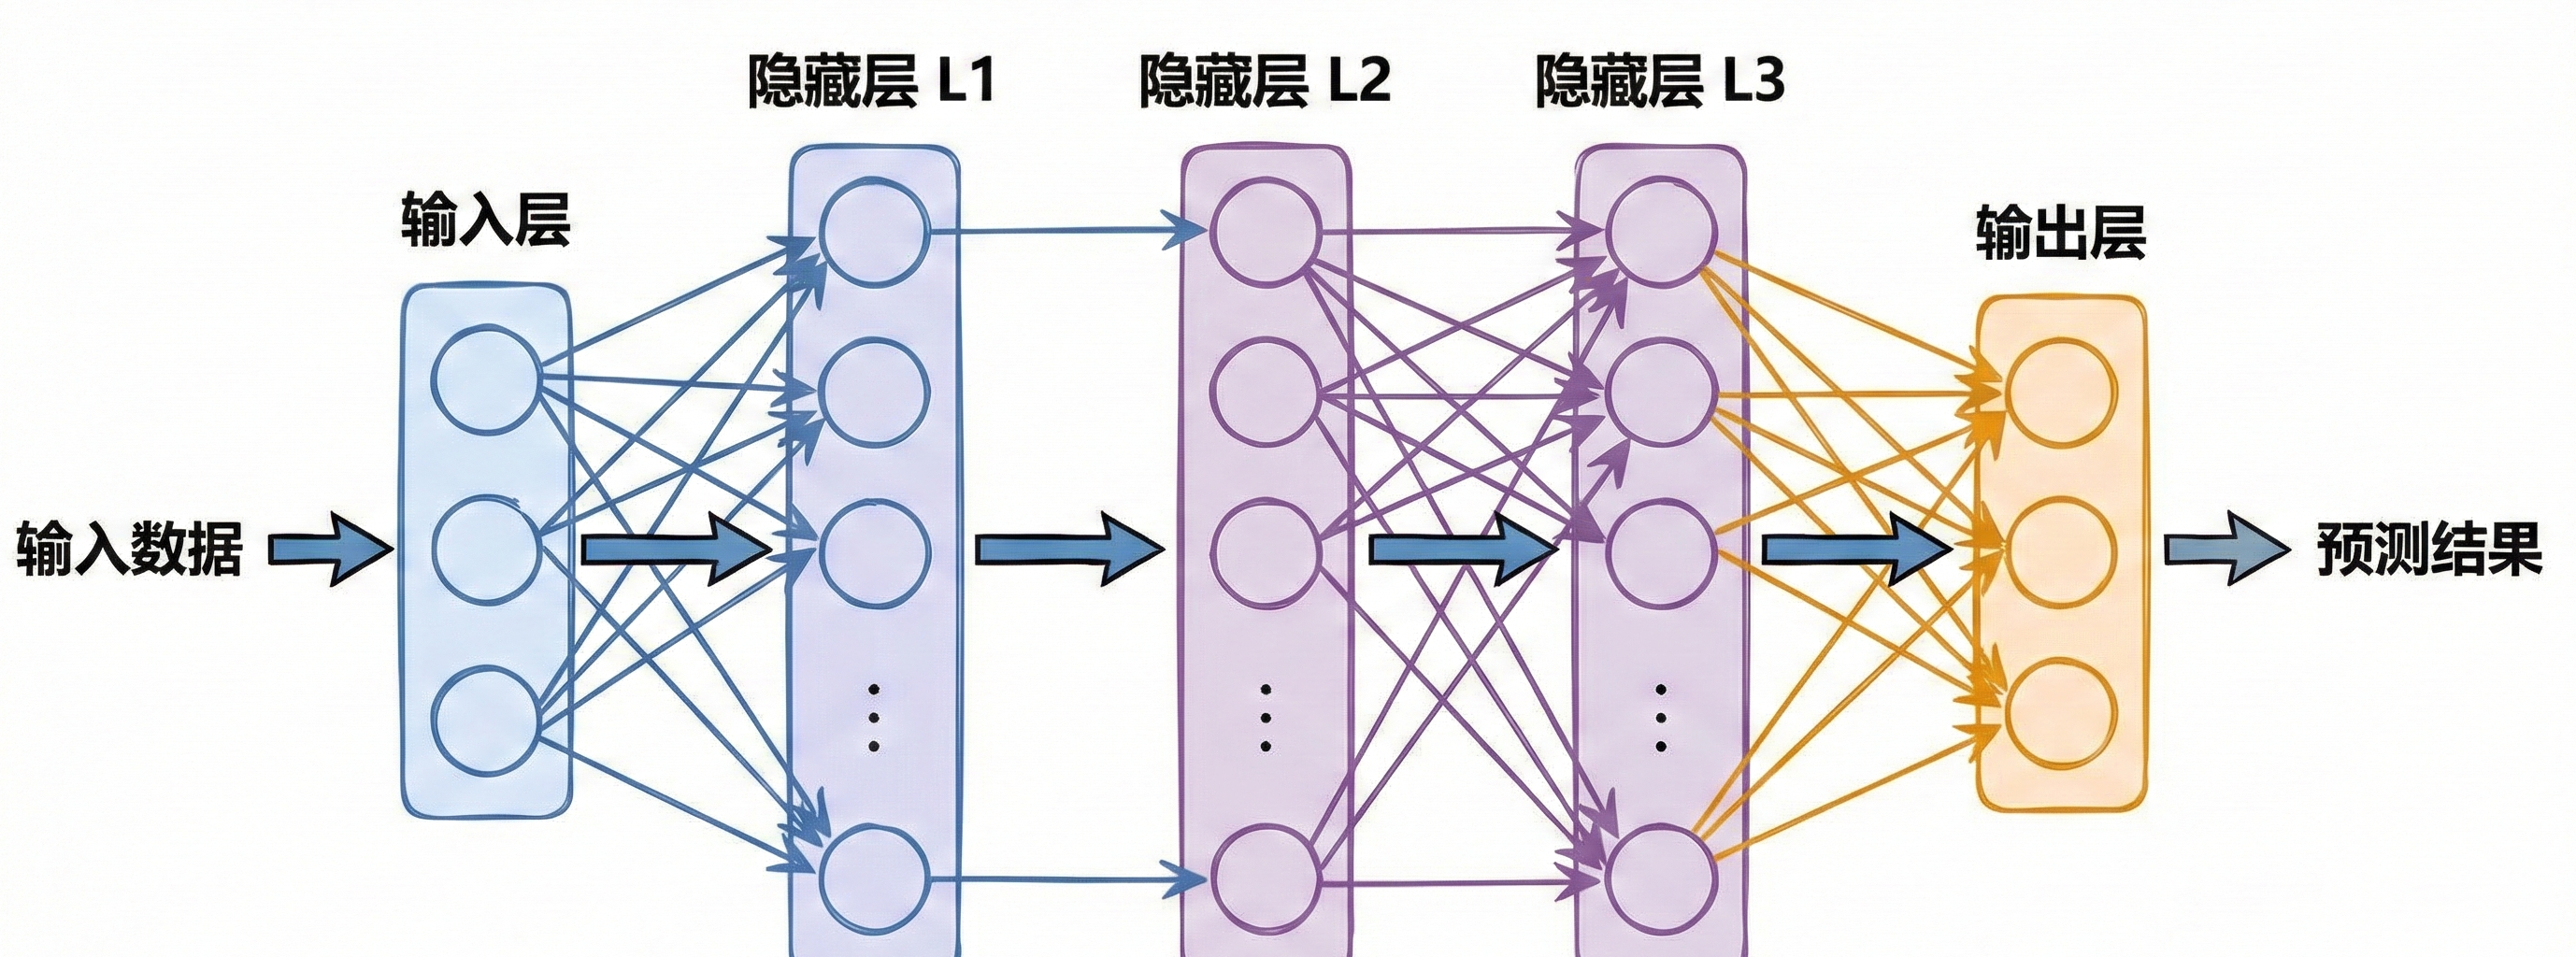
\includegraphics[width=0.75\textwidth]{figures/fig-3-4-1-deep-network-architecture.png}
\caption{\textbf{深度网络分层结构示意图}}
\label{fig:3-4-1-deep-network-architecture}
\end{figure}

\noindent 以图像识别为例。输入是一张照片时,靠近输入的层往往首先捕捉局部的边缘、纹理等低层模式;随着层数加深,这些低层模式会被逐步组合为更稳定的局部结构,再进一步组合为更高层的语义部件,最终形成对"物体类别"等任务目标更直接的表示。可以把它类比为人类的视觉理解过程:先看到线条和色块,再看出形状,最后形成对整体对象的判断。深度网络的分层结构提供了一种可计算的机制,使这种"从局部到整体、从具体到抽象"的表征转化能够在数据上被学习出来,而不是由人预先规定。

\noindent 这也解释了深度学习与传统特征工程路径的关键差异。传统做法往往把"特征提取"与"任务学习"拆成两个阶段:先由人设计特征,再用相对简单的模型去拟合。例如识别农作物是否患病时,可能先手工构造颜色分布、病斑大小数量等特征,再用逻辑回归或支持向量机分类。深度学习把这两件事合并为一个端到端的过程:特征表示与任务目标由同一个损失函数驱动,并通过同一次训练共同得到。换句话说,深度学习的关键不在于层数多本身,而在于它用统一的目标函数与梯度优化,让模型能够在任务约束下自动形成有用的中间表示,从而减少对人工指定"应该看什么特征"的依赖。

\medskip
\noindent \begin{figure}[htbp]
\centering
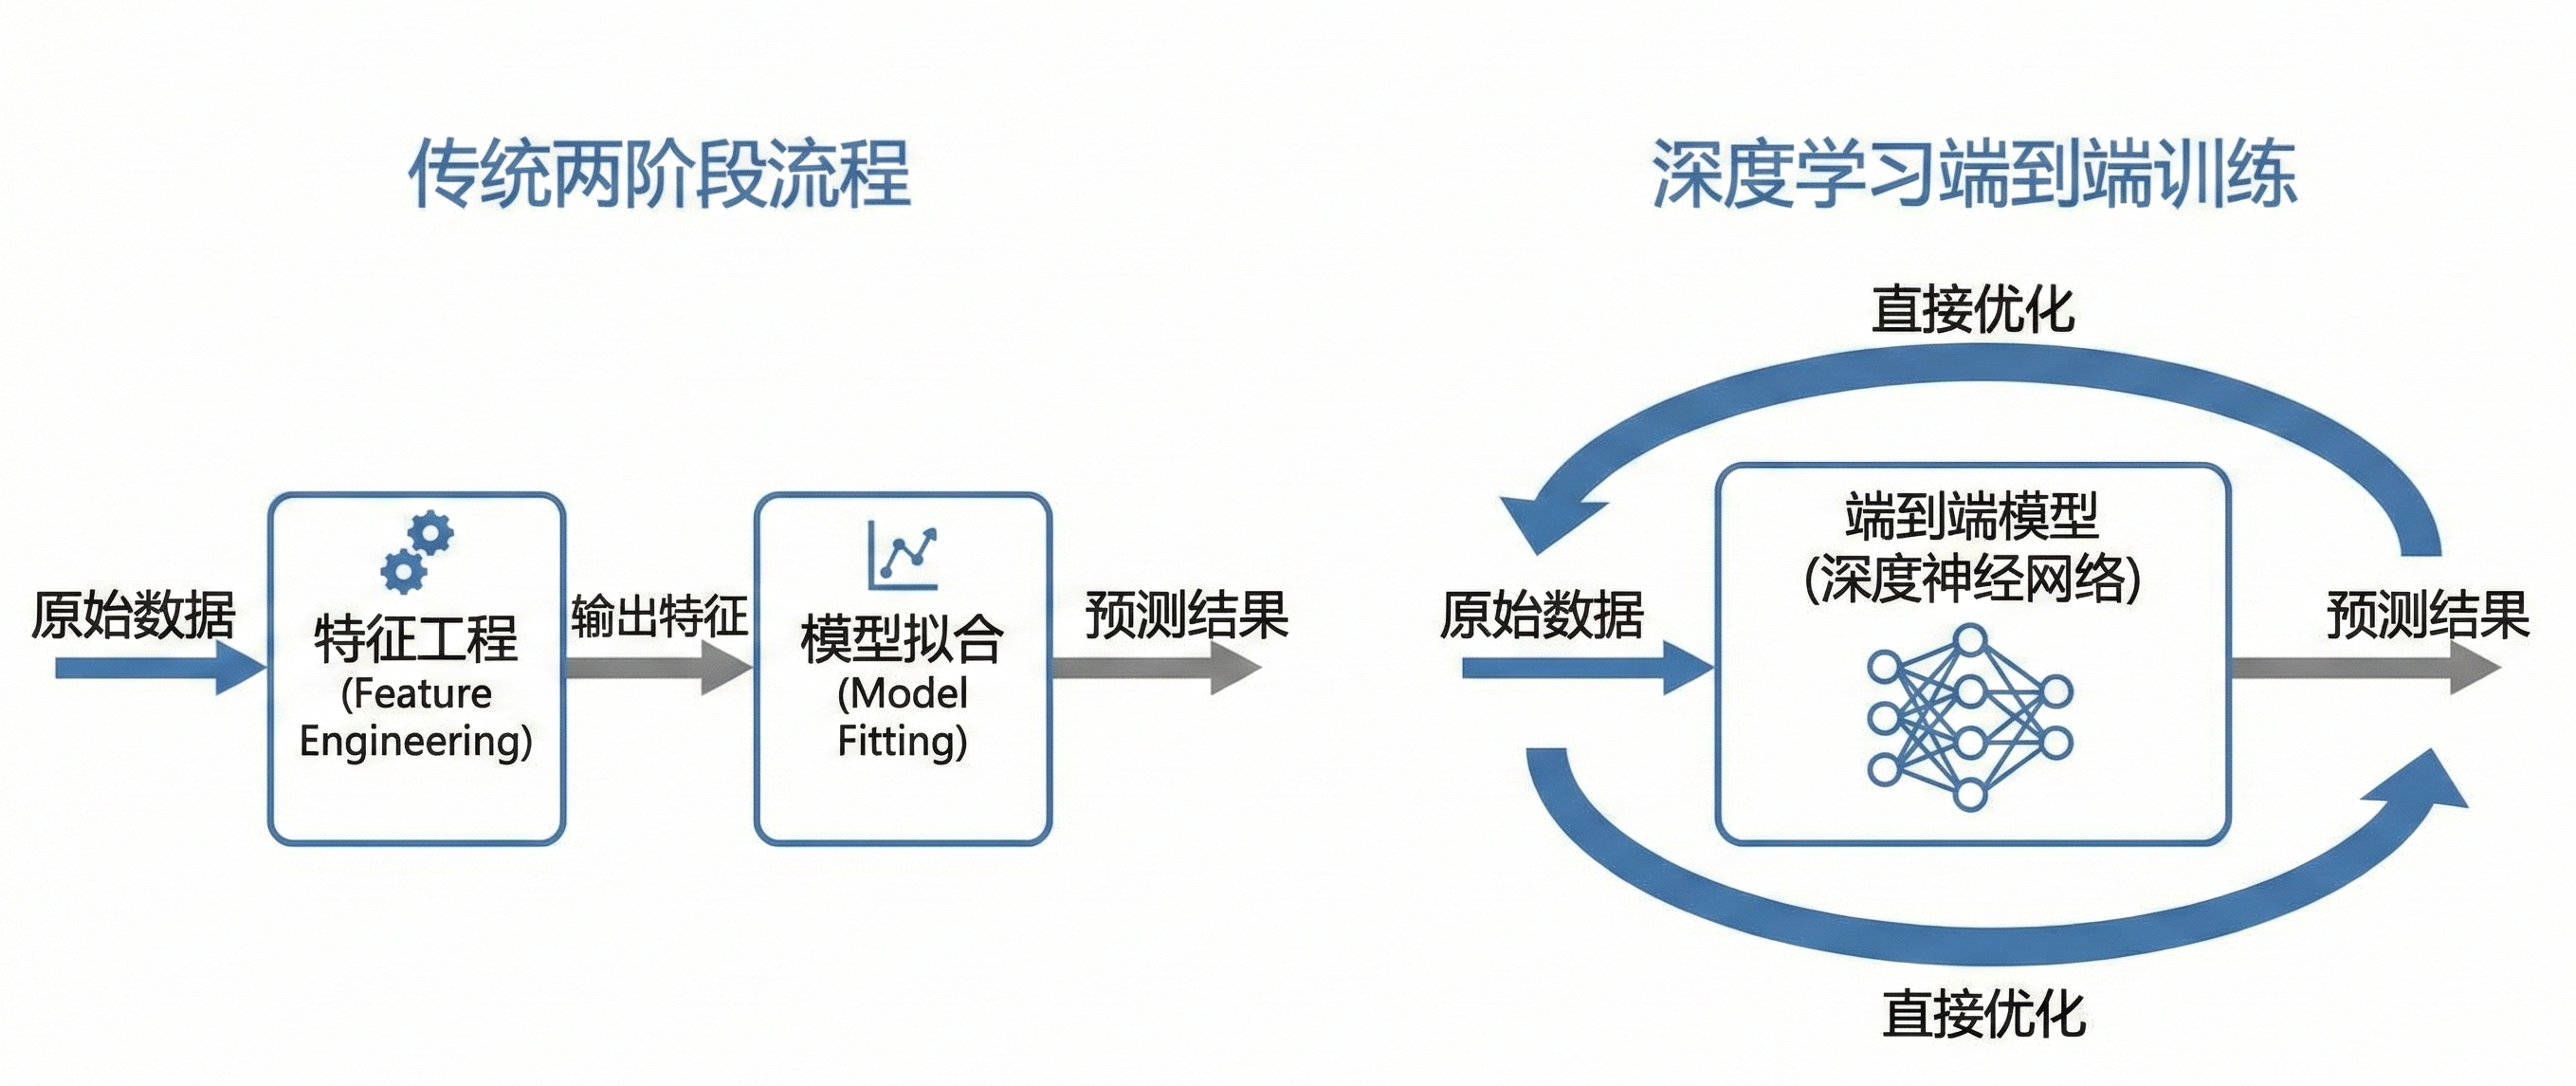
\includegraphics[width=0.75\textwidth]{figures/fig-3-4-2-end-to-end-training.png}
\caption{\textbf{端到端训练与传统两阶段流程对比示意图}}
\label{fig:3-4-2-end-to-end-training}
\end{figure}

\noindent 从训练目标的形式看,深度学习通常同样被写成一个优化问题。以最常见的监督学习为例,给定数据集 $\mathcal D=\{(x_i,y_i)\}_{i=1}^n$,选择损失函数 $L(\cdot,\cdot)$ 来衡量预测 $\hat y_i=f(x_i;\theta)$ 与真实 $y_i$ 的偏差,训练目标是最小化平均损失,并常加入正则项控制复杂度:
\[ \min_{\theta}\; J(\theta)=\frac{1}{n}\sum_{i=1}^n L\big(y_i,f(x_i;\theta)\big)+\lambda\,\Omega(\theta). \]
这一形式与前面3.3节的监督学习在结构上完全一致,差别主要在于此处的 $f(x;\theta)$ 是由多层复合构成的高容量函数族。正因为容量高,深度网络能够拟合更复杂的输入—输出关系,但也更依赖合理的训练策略与泛化控制,否则容易出现训练不稳定或过拟合。深度"为何重要",也可以在这一框架下被理解:一方面,多层复合通常带来更强的表达效率,许多复杂映射若用单层或浅层模型表达,往往需要大量参数,而用多层结构可以通过逐层组合,以更紧凑的方式实现同样的函数;另一方面,许多现实数据具有天然的层级生成或组合结构,例如视觉中的边缘—形状—部件—物体,语言中的词—短语—句法—语义,分层表示为模型提供了更合适的归纳偏好,使其更容易以可复用的组件组织复杂规律。

\noindent 需要注意的是,表达能力强并不自动意味着训练就容易。深度网络训练依赖梯度法,通过反向传播高效计算 $\nabla_\theta J(\theta)$,再用梯度下降或其变体更新参数
\[ \theta\leftarrow \theta-\eta \nabla_\theta J(\theta), \]
其中 $\eta$ 是学习率。对读者而言,此处需要抓住一个核心事实:深度学习并没有绕开传统学习理论的基本约束,它只是把可表示的函数空间扩展得更大,并通过可微分计算图与梯度优化使大规模参数学习成为可能。后续常见的训练技巧(初始化、归一化、正则化、优化器、数据增强等)都可以理解为在这个高容量、强非线性的函数空间里,让梯度优化更稳定,让学到的表示更可泛化。理解了深度学习的这一定位之后,读者就能够在后续章节更自然地接受卷积神经网络、Transformer等具体结构:它们是在同一深度学习框架下,为不同数据形态引入不同的结构偏好与计算方式,从而更高效地学习有用的表示。
\subsubsection*{3.4.2\quad 前向计算与训练机制}

\noindent 深度学习最需要把握的,不是某一种网络结构的细节,而是一套稳定的计算与训练闭环:网络如何把输入变成输出,训练又如何把输出与目标之间的差距反过来变成参数更新。只要这条闭环清晰,后面无论遇到卷积神经网络还是Transformer,都可以把它们看作是在同一训练机制下更换了不同的前向计算模块。实践中的训练过程可以概括为四个环节的循环往复:前向计算把输入映射为输出;损失函数把输出与真实标签之间的差距量化为一个标量;反向传播把这个差距分解为对各层参数的梯度信号;优化器再依据梯度更新参数。训练轮次不断推进,直到性能不再提升或达到预定的停止条件。

\noindent 神经网络的前向计算通常可以概括为线性变换与非线性变换的交替复合。设输入为 $x\in\mathbb R^{d_0}$,记 $h^{(0)}=x$,第 $\ell$ 层的线性部分为
\[ z^{(\ell)} = W^{(\ell)}h^{(\ell-1)} + b^{(\ell)},\]
其中 $W^{(\ell)}\in\mathbb R^{d_\ell\times d_{\ell-1}}$ 是权重矩阵,$b^{(\ell)}\in\mathbb R^{d_\ell}$ 是偏置向量;随后通过激活函数得到
\[ h^{(\ell)}=\phi\!\left(z^{(\ell)}\right).\]
把这些层按顺序串起来,就得到一个整体复合函数 $f(x;\theta)$,其中参数 $\theta=\{W^{(\ell)},b^{(\ell)}\}_{\ell=1}^L$。直观上,这相当于把输入逐层重编码:前几层往往形成更局部、更简单的模式,中间层把这些模式组合成更抽象的表示,最后一层把抽象表示映射为任务需要的输出。以识别农作物病害为例,靠近输入的层可能先对叶片的颜色与纹理敏感;更深的层逐步形成对病斑形状、边界与分布模式的表征;最终输出层将这些表征汇聚为对病害类型及严重程度的判断。

\medskip
\noindent \begin{figure}[htbp]
\centering
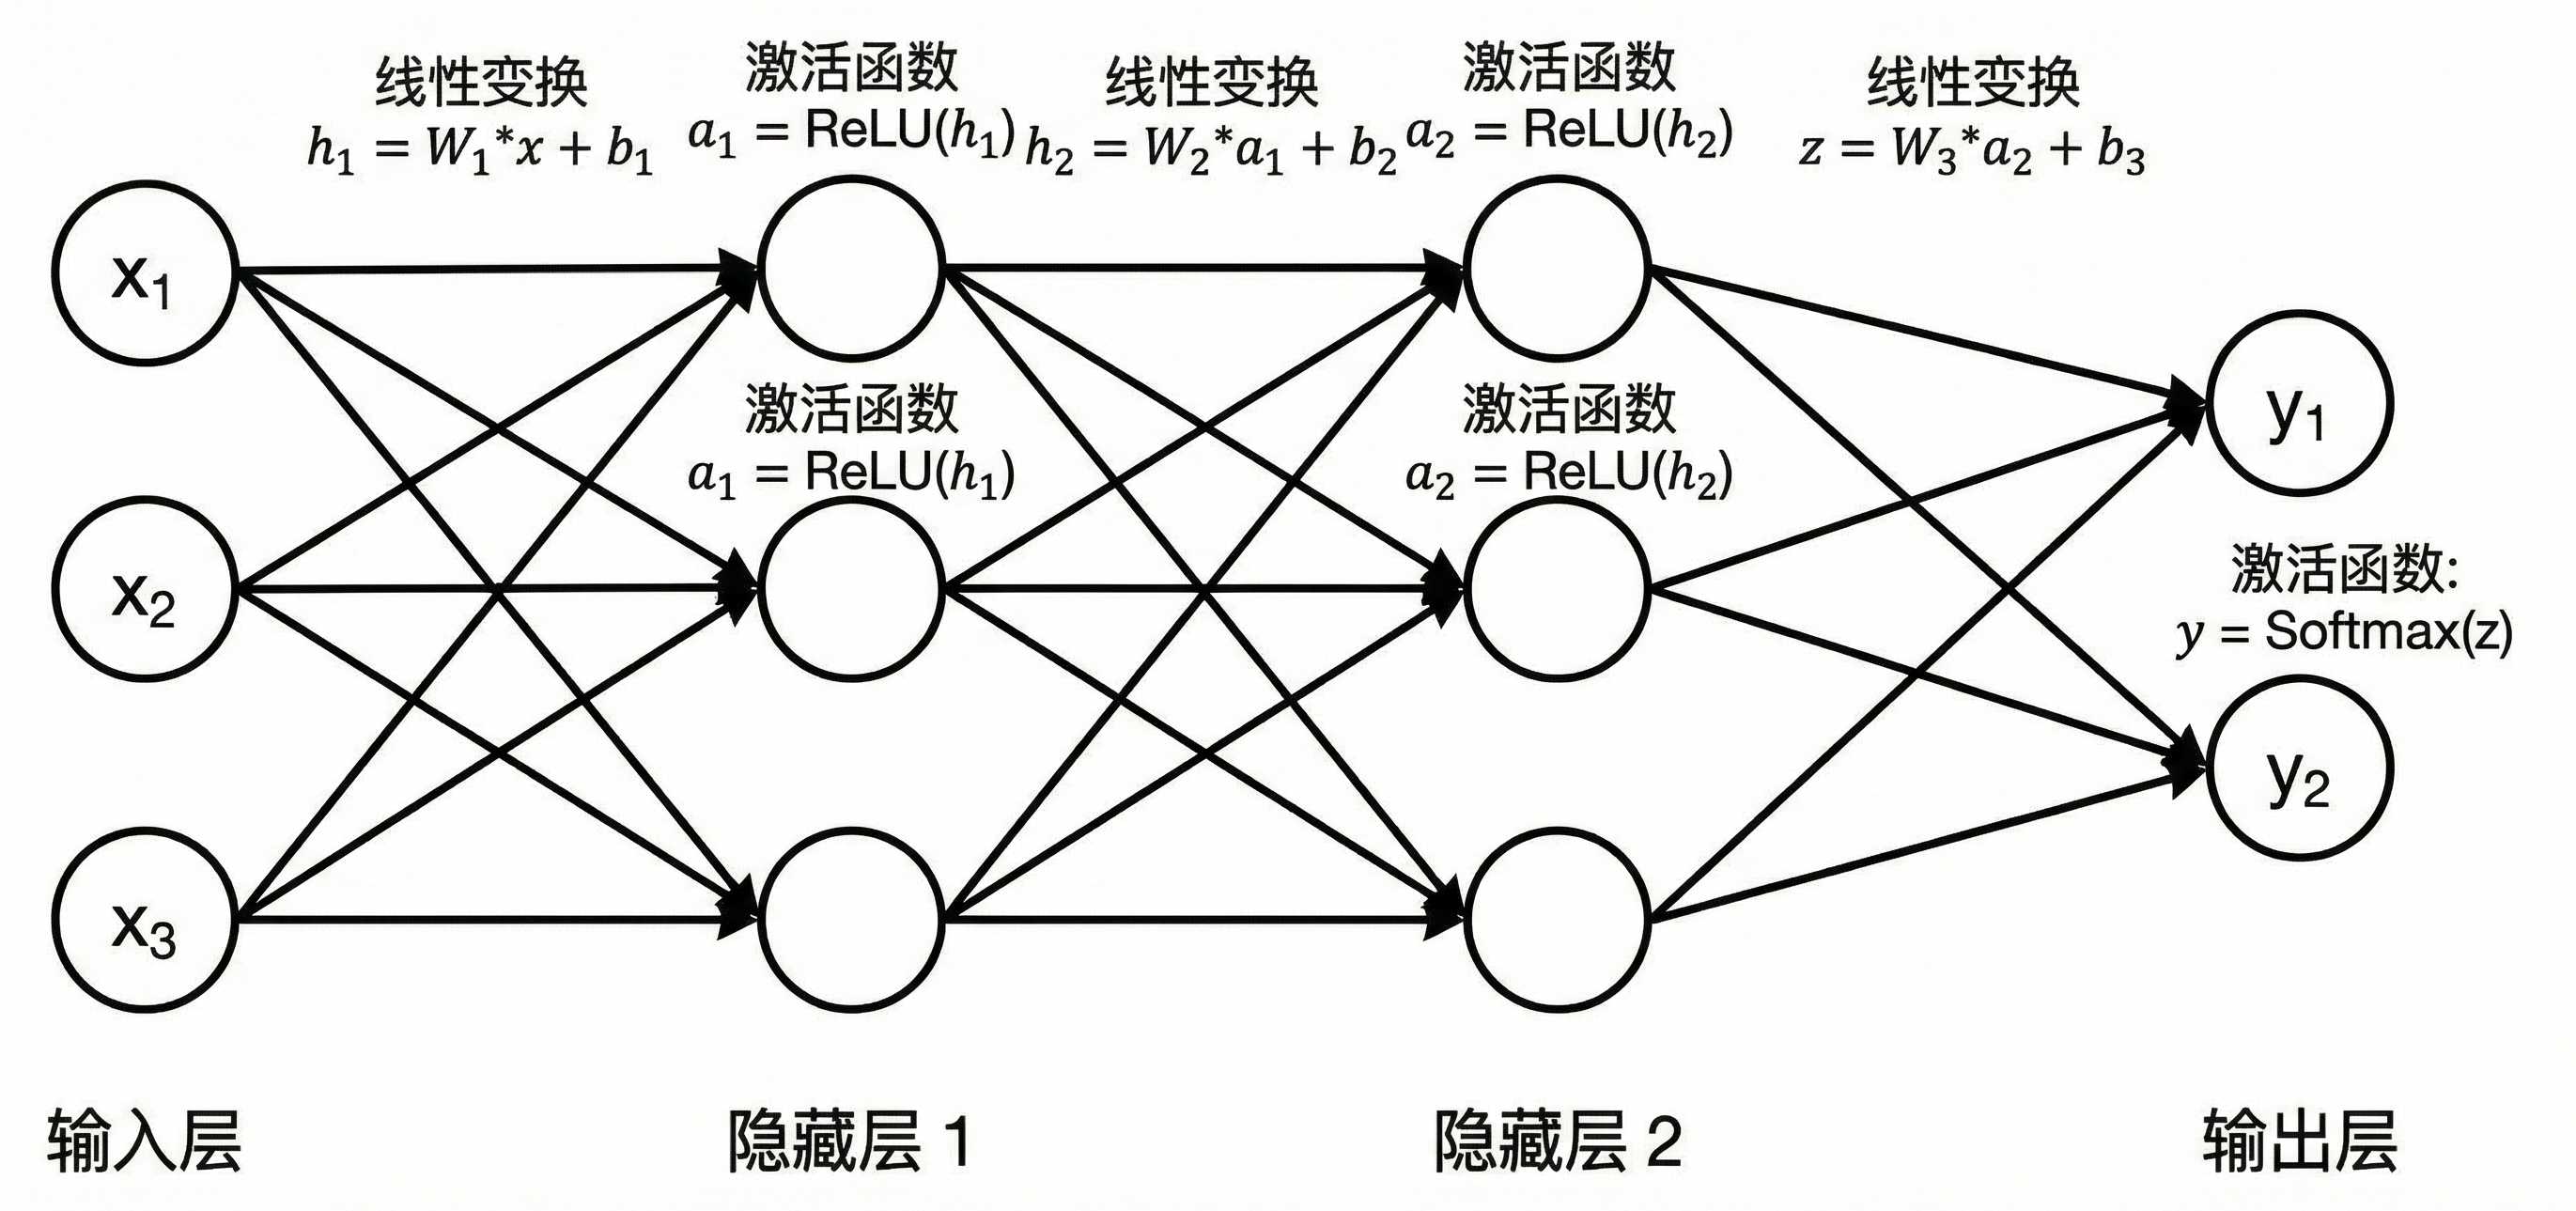
\includegraphics[width=0.75\textwidth]{figures/fig-3-4-3-forward-propagation.png}
\caption{\textbf{神经网络前向计算示意图}}
\label{fig:3-4-3-forward-propagation}
\end{figure}

\noindent 这种"线性变换堆叠很多层"的结构之所以能够表达复杂规律,关键在于非线性激活的引入。如果把所有激活函数 $\phi$ 都去掉,那么多层线性变换的复合仍然等价于一次线性变换,网络再深也只能表达线性关系。非线性提供了"弯折空间",使网络能够表示复杂的非线性函数与非线性决策边界。可以用一个近似的几何类比来理解:如果真实关系是弯曲的,只允许用直线去拟合往往无法贴合;但若允许用多段折线逐段逼近,就可以通过不断增加折点来逼近任意复杂的曲线。激活函数的作用,就是让每一层都有产生一次"折点/弯折"的能力,多层叠加便形成更强的表示能力。常见激活函数包括 ReLU、tanh、sigmoid 等;在训练机制的层面,重要的不是它们的具体形状细节,而是它们使网络从线性模型跃迁为非线性模型。ReLU 之所以最常用,一个直接原因是其形式简单、计算高效,并且在大规模训练中表现稳定。

\noindent 前向计算的最后一步还需要与任务类型对齐,以保证网络输出的语义与训练目标一致。回归问题往往直接输出实数向量 $\hat y$;二分类问题通常输出一个概率 $\hat p\in(0,1)$;多分类问题则输出对各类别的概率分布。对应地,输出层常写为
\[ \hat y = g\!\left(W^{(L)}h^{(L-1)}+b^{(L)}\right),\]
其中 $g$ 的选择取决于任务。二分类常用 sigmoid:
\[ \hat p=\sigma(z)=\frac{1}{1+e^{-z}},\]
多分类常用 softmax:
\[ \hat p_k=\frac{e^{z_k}}{\sum_{j=1}^K e^{z_j}}.\]
把输出解释为概率的意义在于,训练目标可以自然地写成"让真实标签在模型输出分布下尽可能大",从而得到对数似然与交叉熵等标准形式,使训练过程具有清晰的统计解释与可比较的评价尺度。

\noindent 有了与任务对齐的输出语义,训练目标就可以被明确地写成一个优化问题。给定样本 $(x_i,y_i)$,网络前向得到预测 $\hat y_i=f(x_i;\theta)$,损失函数 $L(y_i,\hat y_i)$ 衡量预测与真实的差异。训练的目标是最小化训练集上的平均损失,必要时加入正则项以控制复杂度:
\[ J(\theta)=\frac{1}{n}\sum_{i=1}^n L\big(y_i,f(x_i;\theta)\big)+\lambda\Omega(\theta),\qquad \theta^\ast=\arg\min_\theta J(\theta).\]
在这一步上,监督学习与深度学习并没有本质差异:差异主要来自 $f(\cdot;\theta)$ 的函数族更复杂、参数更多、表达能力更强,因此既能拟合更丰富的模式,也更需要稳定的训练策略与有效的泛化控制。

\noindent 真正让深度网络可训练的是反向传播与基于梯度的优化。反向传播并不是另一套独立的学习规则,它只是把链式法则系统化地应用到计算图上,用高效的方式计算出 $\nabla_\theta J(\theta)$。一次参数更新可以写成
\[ \theta \leftarrow \theta-\eta \nabla_\theta J(\theta),\]
其中 $\eta$ 是学习率。直观地理解,前向计算告诉我们网络当前输出什么、偏差在哪里;反向传播告诉我们这些偏差应当分别归因到哪些参数上,以及每个参数沿哪个方向微调最能让损失下降。梯度就是这种"应该怎么改"的定量化信号。为了把反向传播在"传什么"说清楚,可以用误差信号的传播来描述。对第 $\ell$ 层,定义该层线性输出 $z^{(\ell)}$ 上的误差信号
\[ \delta^{(\ell)}=\frac{\partial J}{\partial z^{(\ell)}}.\]
则参数梯度满足
\[ \frac{\partial J}{\partial W^{(\ell)}}=\delta^{(\ell)}(h^{(\ell-1)})^\top,\qquad \frac{\partial J}{\partial b^{(\ell)}}=\delta^{(\ell)},\]
而误差信号在层与层之间的传播满足
\[ \delta^{(\ell)}=\big((W^{(\ell+1)})^\top \delta^{(\ell+1)}\big)\odot \phi'\!\left(z^{(\ell)}\right),\]
其中 $\odot$ 表示按元素相乘。这个关系式表达的含义很直接:上一层的误差来自下一层误差的回传,再乘上本层激活函数在当前位置的导数,刻画"本层输出的微小变化会对整体损失造成多大影响"。反向传播之所以高效,是因为它把整网的梯度计算分解为局部的矩阵运算,并复用前向阶段缓存的中间量,避免了对同一子表达式的重复求导与重复计算。

\medskip
\noindent \begin{figure}[htbp]
\centering
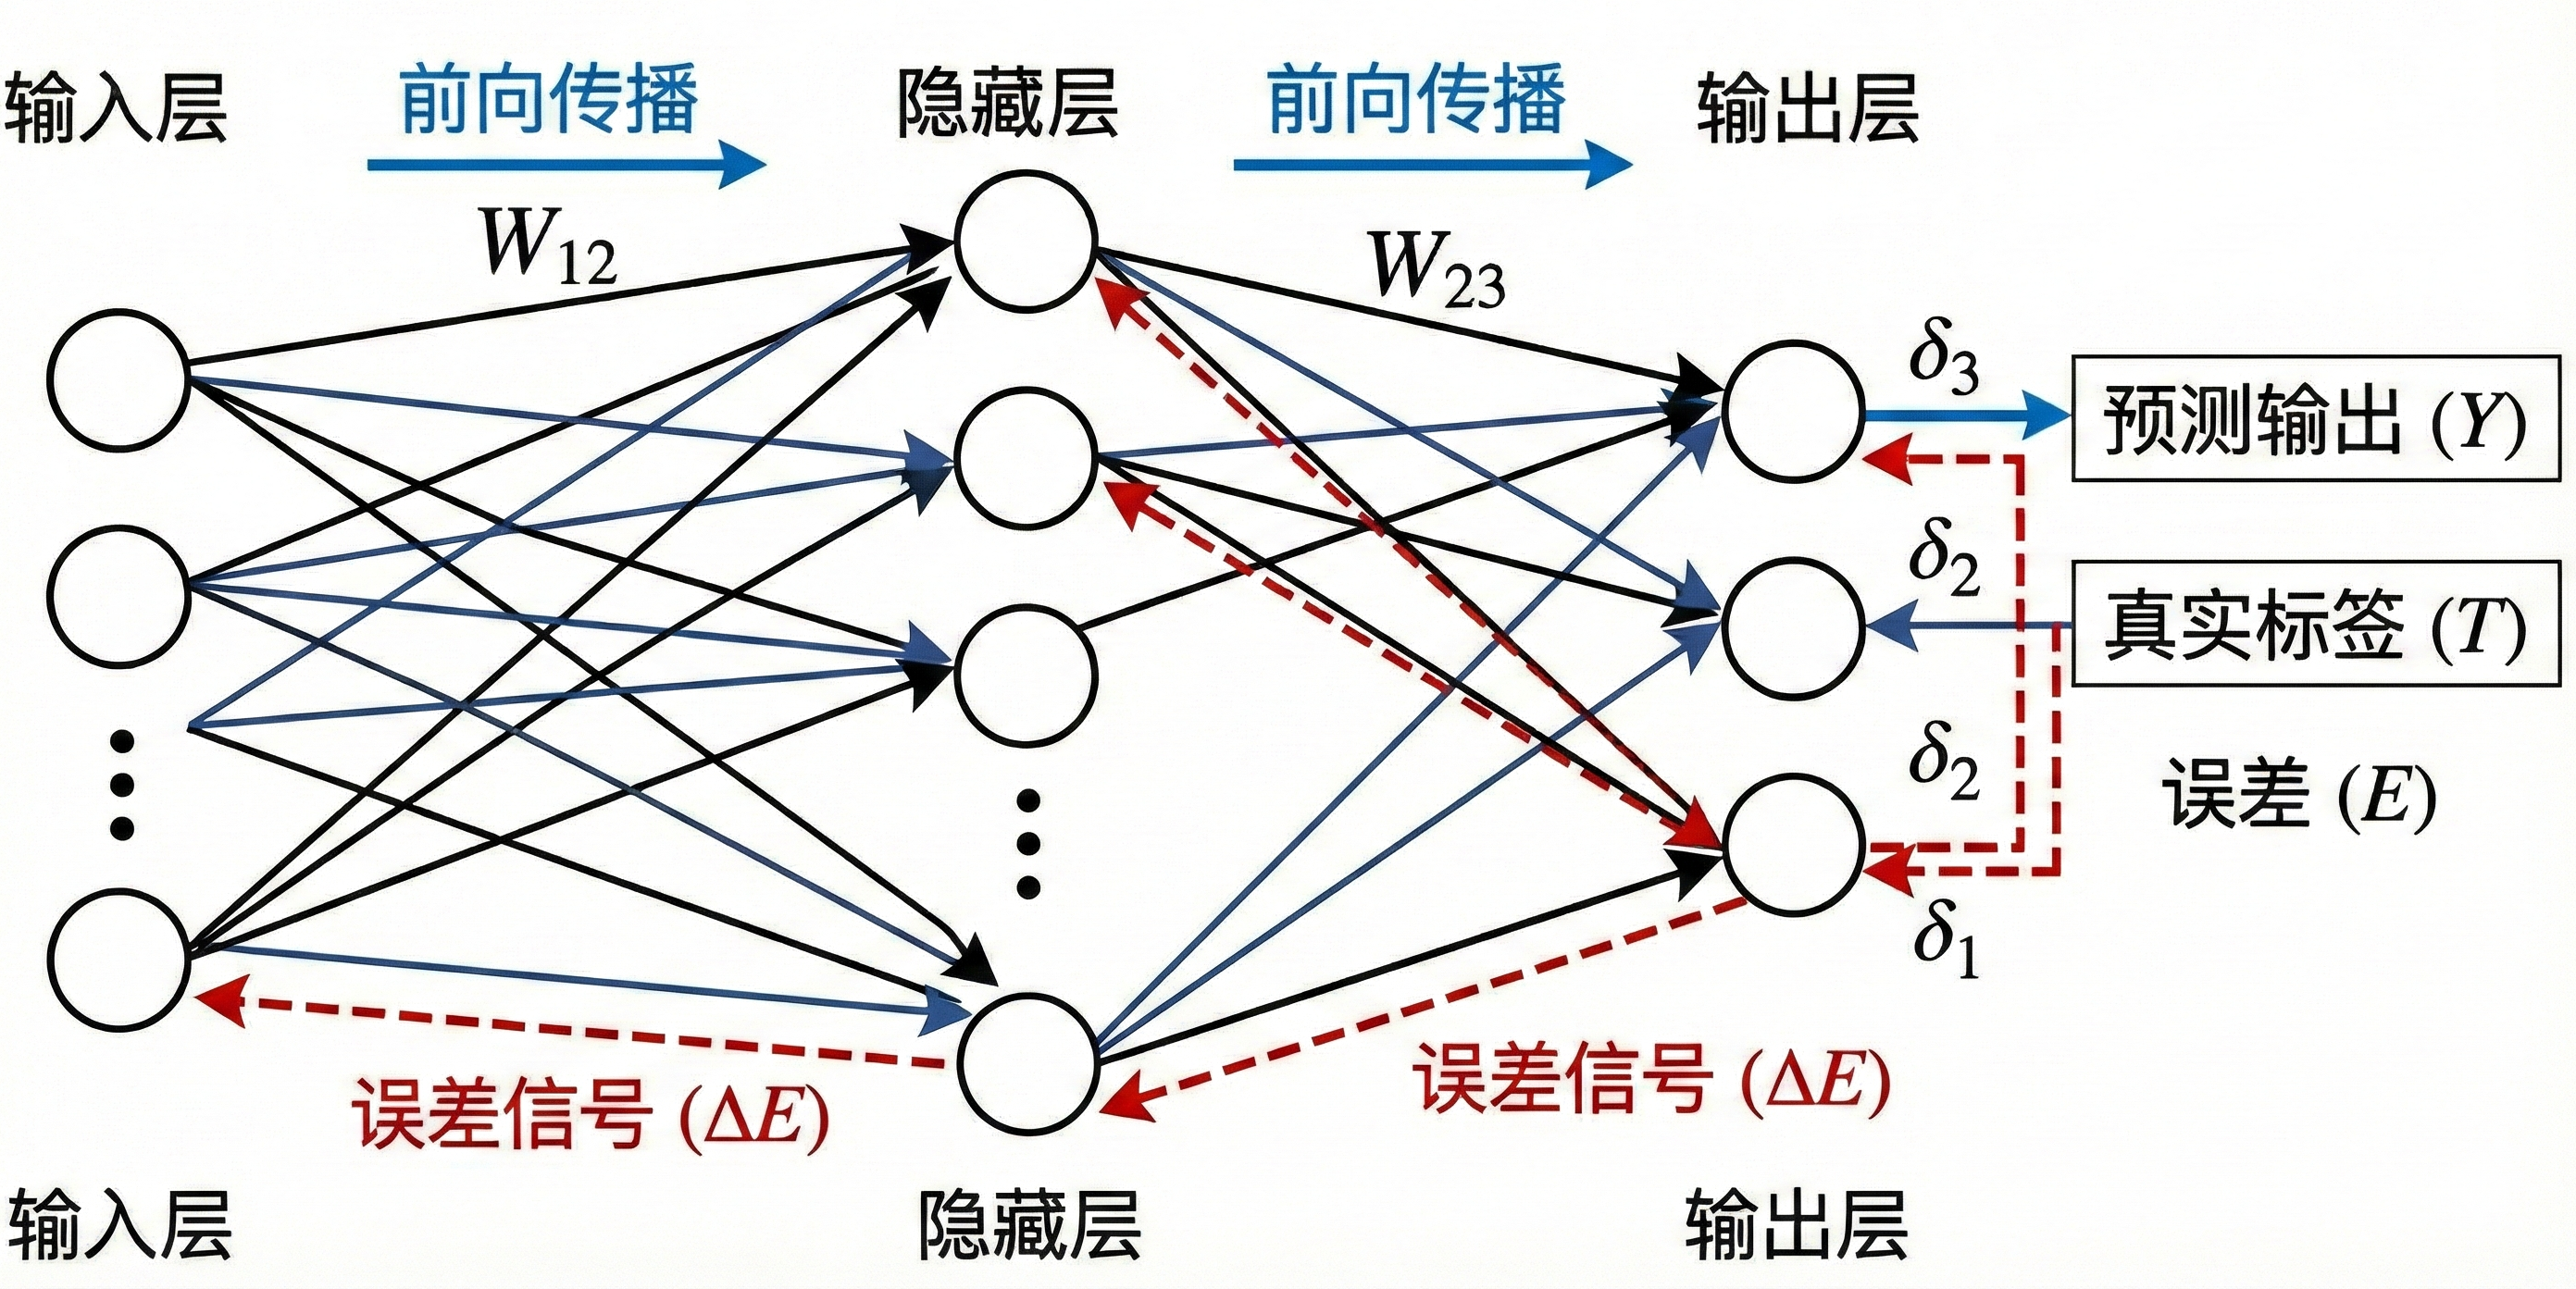
\includegraphics[width=0.75\textwidth]{figures/fig-3-4-4-backpropagation.png}
\caption{\textbf{反向传播误差信号回传示意图}}
\label{fig:3-4-4-backpropagation}
\end{figure}

\noindent 在工程实践中,很少使用全量梯度下降,而更常用小批量随机梯度下降:将数据划分为批次 $B$,每次用一个批次近似整体梯度
\[ \nabla_\theta J(\theta)\approx \frac{1}{|B|}\sum_{i\in B}\nabla_\theta L\big(y_i,f(x_i;\theta)\big),\]
然后执行一次参数更新。这样做一方面显著提高计算效率,使训练可以在有限显存与时间预算下推进;另一方面,批次梯度所带来的随机噪声在一定程度上反而有助于优化过程跳出不佳的局部区域或平坦区域,从而更容易获得更好的解。优化器可以是基础的随机梯度下降,也可以加入动量或自适应学习率机制(如 Adam)以改善收敛速度与稳定性,但在训练机制的层面,它们做的仍是同一件事:利用梯度信息确定更新方向,并用不同的规则调节更新幅度、平滑噪声与控制训练动态。

\noindent 归纳起来,网络结构改变的是前向计算的具体形式与所引入的归纳偏置;但"前向—损失—反向—更新"的训练闭环保持不变。理解这一点,读者在后续学习卷积神经网络的卷积算子或 Transformer 的注意力算子时,关注点就会自然落在:新的前向模块如何改变信息的流动与表示的组织方式,而不是误以为需要重新学习一套完全不同的训练逻辑。
\subsubsection*{3.4.3\quad 卷积神经网络基础}

\noindent 卷积神经网络之所以适合处理图像,并不因为它采用了与其他神经网络完全不同的训练机制。它同样遵循前向计算、损失函数、反向传播、梯度更新的训练闭环。卷积神经网络的关键变化发生在前向计算的结构设计上:它把"局部模式可以在整幅图上反复出现"这一经验写进网络结构,使网络在学习时天然倾向于提取边缘、角点、纹理等局部结构,并把这些结构在空间上的分布以特征图的形式保留下来。图\ref{fig:cnn-sliding-window}给出了一个更贴近"卷积在做什么"的示意:左侧输入图像存在明显的明暗分界;中间展示卷积核在输入上以滑动窗口方式做局部点积(滑动窗口 \& 点积);图中用两组方向性边缘检测核(示例为 Sobel $X$ 与 Sobel $Y$)分别对输入做卷积,从而得到两张输出特征图。可以看到,其中一张特征图在分界处出现高亮响应带,说明该方向的卷积核与图像中的边缘方向匹配;另一张特征图整体接近零,说明在该输入下,与其对应方向的边缘并不明显。右侧进一步把两个方向的边缘响应进行融合,得到更稳定的边缘表征。

\begin{figure}[htbp]
\centering
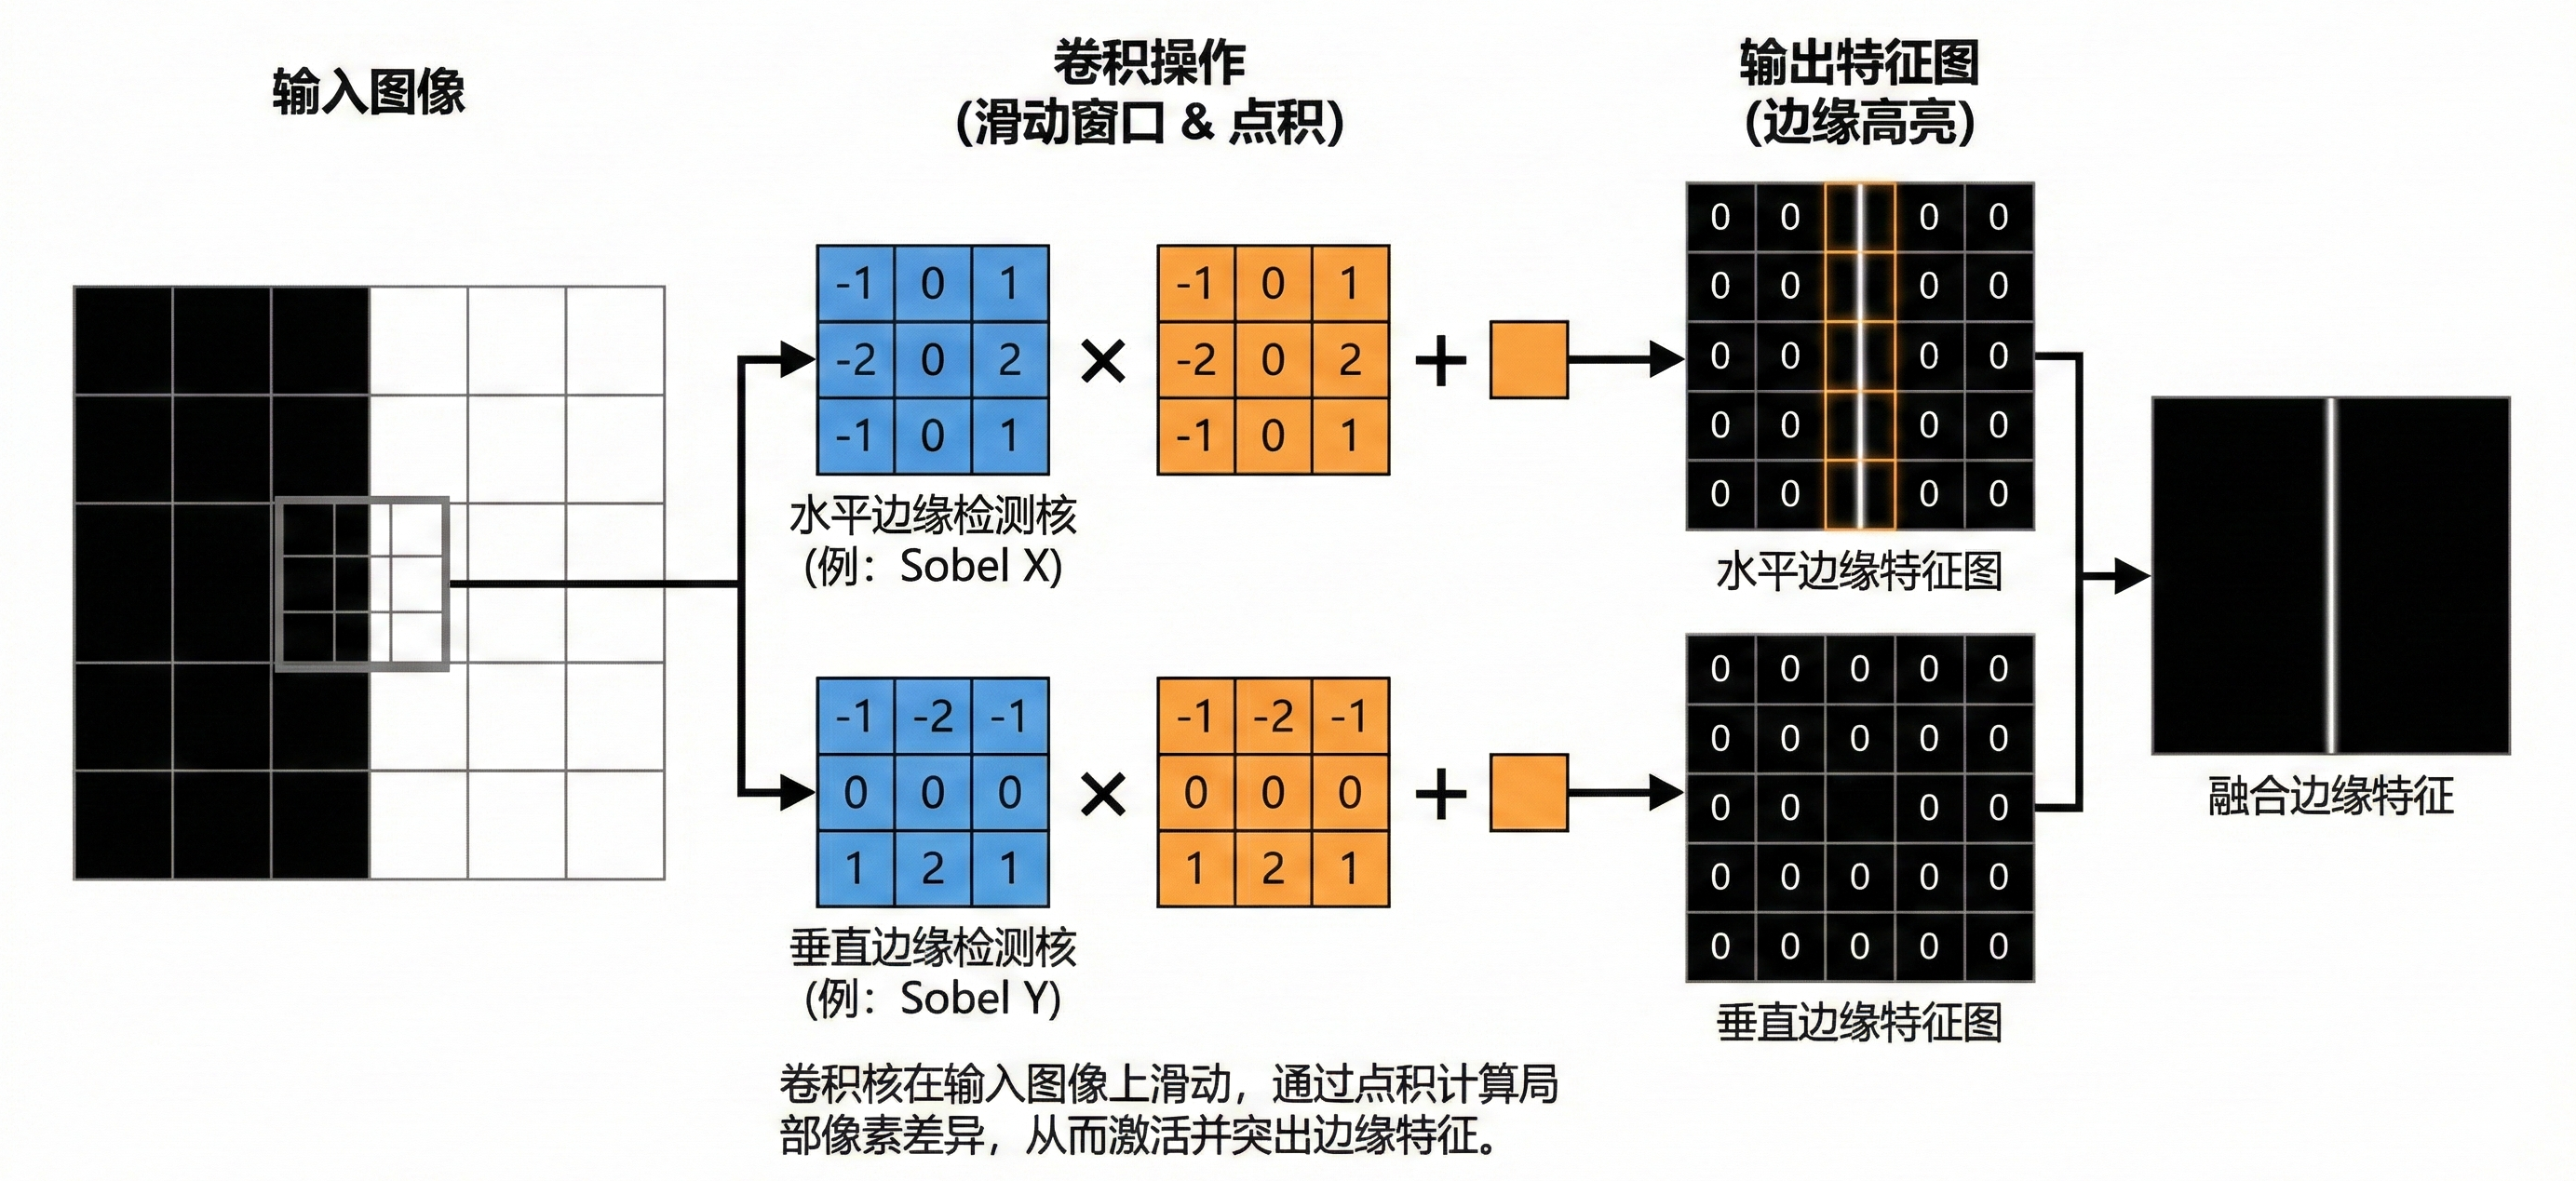
\includegraphics[width=0.9\textwidth]{figures/fig-cnn-sliding-window}
\caption{卷积用于边缘检测的直观示意:卷积核在输入图像上滑动,在每个局部窗口内做点积得到响应;使用两组方向性边缘检测核(示例为 Sobel $X$ 与 Sobel $Y$)可分别产生两张方向特征图,其中与输入边界方向一致的特征图在边界处出现高亮响应带;将两张方向特征图融合可得到更完整的边缘特征。}
\label{fig:cnn-sliding-window}
\end{figure}

\noindent 在最常见的二维情形中,输入是一张二维网格(例如灰度图像)$X\in\mathbb R^{H\times W}$。卷积层用一个小的权重矩阵(卷积核)$W\in\mathbb R^{k\times k}$在输入上滑动。每次滑动,卷积核只覆盖输入图像的一块局部区域,并在该局部窗口上做加权求和,得到输出特征图 $Y\in\mathbb R^{(H-k+1)\times(W-k+1)}$:
\[ Y_{i,j}=\sum_{u=0}^{k-1}\sum_{v=0}^{k-1}W_{u,v}\,X_{i+u,\,j+v}+b,\]
其中 $b$ 是偏置项。随后通常还会接一个非线性激活函数 $\phi(\cdot)$ 得到
\[ H_{i,j}=\phi(Y_{i,j}).\]
若输入是多通道(例如 RGB 图像),则 $X\in\mathbb R^{H\times W\times C}$。此时卷积核在空间维度仍是 $k\times k$,但同时覆盖 $C$ 个通道,输出每个位置的值来自对所有通道对应局部窗口的加权汇总;多个卷积核会产生多个输出通道,从而形成更丰富的特征表示。就本节的目的而言,理解单通道卷积的核心计算与"滑动窗口点积产生特征图"的含义,已足以把握卷积神经网络的基本思想。

\noindent 卷积计算的直观意义,可以直接借助图\ref{fig:cnn-sliding-window}中"方向性边缘检测核"的对比来理解。图中给出两组 $3\times3$ 的边缘检测核(示例为 Sobel $X$ 与 Sobel $Y$),它们的系数结构体现了"对某一方向的像素差异更敏感"的偏好:当卷积核覆盖的局部窗口跨越明暗分界时,窗口两侧像素值差异显著,点积结果会出现较大的幅度,从而在输出特征图的对应位置形成高亮响应;当局部窗口落在灰度相对均匀的区域时,加权求和相互抵消,输出更接近零。因此,在图\ref{fig:cnn-sliding-window}中,与输入边界方向相匹配的那一路卷积会在分界处产生一条明显的高亮带,而另一方向由于缺乏对应的边缘结构,响应整体较弱。进一步地,将两路方向响应进行融合,可以得到更完整、更鲁棒的边缘表征,这也是实践中常见的做法:先用不同卷积核提取互补的局部结构,再在后续层中把这些结构组合成更高层次的形状与语义。

\noindent 从结构角度看,卷积层的优势可以概括为"用局部计算生成空间化表示"。每一个输出位置只由输入的一小块区域决定,这一小块区域称为感受野。对上式而言,$Y_{i,j}$ 只依赖 $X$ 的一个 $k\times k$ 子矩阵;这正对应图\ref{fig:cnn-sliding-window}中以滑动窗口标出的局部点积过程。局部计算来自对图像数据的基本判断:边缘是局部灰度突变,纹理是局部重复模式,角点是局部方向变化。与其让网络在第一层就把整张图像的所有像素一次性混合,不如先在局部范围内检测可复用的小模式,再逐层把这些小模式组合成更大的结构。局部连接还会显著降低参数规模:若用全连接层把 $H\times W$ 个像素直接映射到 $m$ 个隐藏单元,参数量是 $mHW$ 量级;而卷积层对单个卷积核只需要 $k^2$ 个参数(多通道时为 $k^2C$),从而更容易在有限数据下学习到可泛化的局部规律。

\noindent 为了把卷积的"滑动窗口加权求和"落到可计算的步骤上,可以给出一个可手算的最小例子。考虑一个 $3\times3$ 的输入矩阵
\[ X=\begin{pmatrix} 1&2&0\\ 0&1&3\\ 2&1&1 \end{pmatrix},\]
取一个 $2\times2$ 卷积核
\[ W=\begin{pmatrix} 1&0\\ 0&-1 \end{pmatrix},\quad b=0.\]
采用步幅 $1$、无填充,则输出 $Y$ 为 $2\times2$。逐位置计算:左上角窗口为 $\begin{pmatrix}1&2\\0&1\end{pmatrix}$,因此
\[ Y_{0,0}=1\cdot 1+0\cdot 2+0\cdot 0+(-1)\cdot 1=0;\]
右上角窗口为 $\begin{pmatrix}2&0\\1&3\end{pmatrix}$,因此
\[ Y_{0,1}=1\cdot 2+0\cdot 0+0\cdot 1+(-1)\cdot 3=-1;\]
左下角窗口为 $\begin{pmatrix}0&1\\2&1\end{pmatrix}$,因此
\[ Y_{1,0}=1\cdot 0+0\cdot 1+0\cdot 2+(-1)\cdot 1=-1;\]
右下角窗口为 $\begin{pmatrix}1&3\\1&1\end{pmatrix}$,因此
\[ Y_{1,1}=1\cdot 1+0\cdot 3+0\cdot 1+(-1)\cdot 1=0.\]
汇总得到
\[ Y=\begin{pmatrix} 0&-1\\ -1&0 \end{pmatrix}.\]
如果再接一个 ReLU 激活 $\phi(t)=\max(0,t)$,则负响应会被截断为 0。这个例子的目的不是追求某个任务的"正确输出",而是让读者明确:卷积层输出的每一个位置,本质上就是卷积核在对应局部窗口上的一次点积与加权求和;当滑动窗口跨越某类局部结构(例如明暗分界或特定方向的梯度变化)时,卷积核会产生显著响应,并把这种响应以"特征图上的高值区域"标注出来。图\ref{fig:cnn-sliding-window}中的边缘高亮带,正是这种局部响应在方向性边缘检测核与含边界输入这一组合下的直观呈现。
\subsubsection*{3.4.4\quad Transformer 基础}

\medskip
\begin{figure}[htbp]
\centering
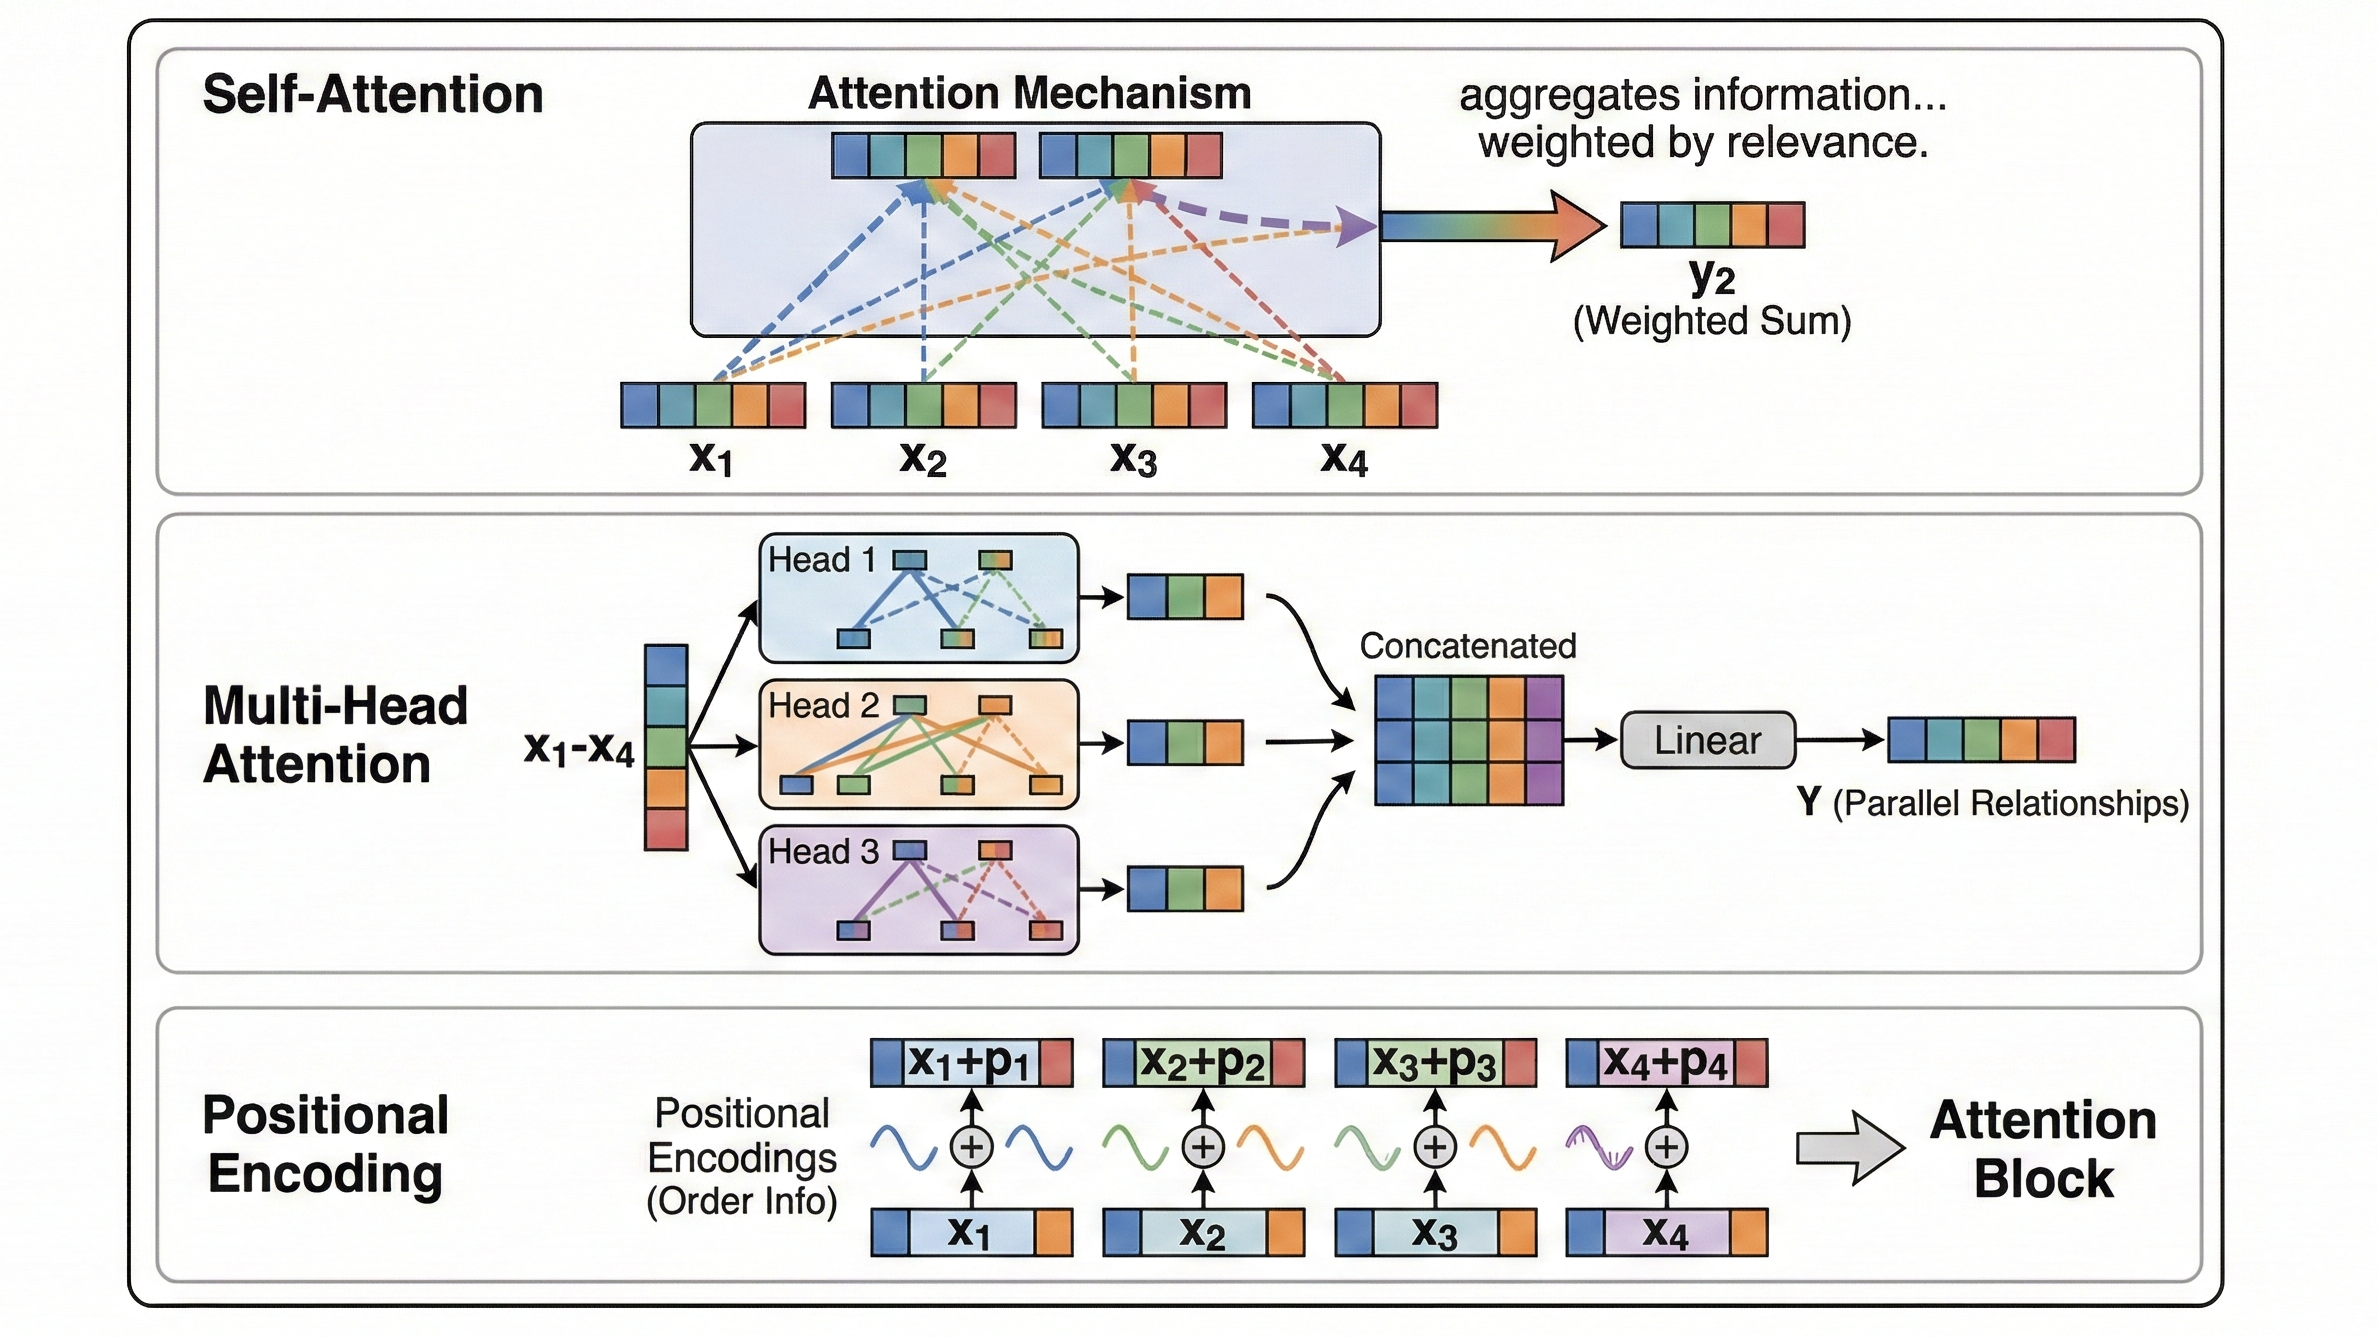
\includegraphics[width=0.9\textwidth]{figures/fig-transformer-attention}
\caption{缩放点积注意力(scaled dot-product attention)的计算流程:由输入生成查询 $Q$、键 $K$、值 $V$,计算相似度并缩放,经 softmax 得到注意力权重,再用权重对 $V$ 做加权求和得到输出。}
\label{fig:transformer-attention}
\end{figure}
\medskip

\noindent 图~\ref{fig:transformer-attention}~展示的并不是完整 Transformer 的所有组件,而是其最核心、最基础的运算单元:缩放点积注意力。图中左侧给出三类输入张量:查询(Query, $Q$)、键(Key, $K$)和值(Value, $V$)。注意力的第一步是用查询去"匹配"键:对每个查询向量与所有键向量计算点积相似度,并按维度做缩放(Dot Product \& Scaling),得到相关性分数矩阵;第二步用 softmax 将分数归一化为注意力权重(Attention Weights),图中以热力图形式呈现,表示"每个查询位置对各键位置分配了多少关注";第三步用这些权重对值向量做加权求和(Weighted Sum),得到输出(Output)。因此,注意力的本质可以概括为:用 $Q$ 与 $K$ 计算"该看哪里",再用该权重对 $V$ 汇聚"要拿什么信息",从而实现跨位置的信息融合。

\noindent Transformer 与循环网络、卷积网络的本质区别,在于信息交互的路径。循环网络的信息需要沿时间步逐步传递,长距离依赖往往意味着长路径;卷积网络的信息主要在局部邻域内传播,想"看到"很远的位置通常需要堆叠很多层以扩大感受野。Transformer 通过注意力机制让任意两个位置在一次计算中直接交互,从而把"全局依赖"变成一次可并行的矩阵运算。设输入序列长度为 $n$,每个位置的表示维度为 $d$,把输入堆叠成矩阵 $X\in\mathbb R^{n\times d}$,其中第 $i$ 行 $x_i^\top$ 表示第 $i$ 个 token 的向量表示;token 可以是词、子词、帧或图像 patch 等基本单元。注意力的核心思想是:对每个位置 $i$,模型会在所有位置 $j$ 上分配权重,再把各位置的表示按权重加权求和,从而得到位置 $i$ 的新表示;可以把它理解为"位置 $i$ 在更新自己的表示时,会去全序列范围内借信息,但借多少由相关性决定"。

\noindent 在计算上,Transformer 先把同一个输入 $X$ 通过三组线性映射生成查询、键、值:
\[ Q=XW_Q,\qquad K=XW_K,\qquad V=XW_V,\]
其中 $W_Q,W_K,W_V\in\mathbb R^{d\times d_k}$,因此 $Q,K,V\in\mathbb R^{n\times d_k}$。直观地看,$q_i$ 表示位置 $i$"需要什么信息"的查询表达,$k_j$ 表示位置 $j$"具有什么信息特征"的标识,$v_j$ 则是位置 $j$ 实际可被汇聚的内容。然后对任意两个位置 $i,j$,以点积 $q_i^\top k_j$ 衡量相关性,并做缩放与 softmax 归一化得到注意力权重矩阵
\[ A=\mathrm{softmax}\!\left(\frac{QK^\top}{\sqrt{d_k}}\right),\qquad A\in\mathbb R^{n\times n},\]
其中 $A_{i,j}$ 表示在更新位置 $i$ 的表示时对位置 $j$ 的关注程度;最后用这些权重对 $V$ 做加权汇总:
\[ \mathrm{Attn}(X)=AV,\qquad \mathrm{Attn}(X)\in\mathbb R^{n\times d_k}.\]
图~\ref{fig:transformer-attention}~中"Dot Product \& Scaling $\rightarrow$ Softmax $\rightarrow$ Attention Weights $\rightarrow$ Weighted Sum"的流程正对应上述公式:缩放点积给出相关性分数,softmax 把分数转成可解释的权重分布,随后对 $V$ 的加权求和产生输出。由于权重是对所有位置分配的,注意力不是"选一个位置",而是"以分布的形式融合多处信息",因此它既能表达局部依赖,也能表达长距离依赖。

\noindent 但序列中的相关性往往不止一种,仅用一套相似度空间去衡量所有关系会受到表达瓶颈限制。以语言为例,相关性可能来自语义相近、语法依赖、指代关系或主题一致等不同维度;以视觉 patch 序列为例,相关性可能来自局部纹理相似、同一物体的不同部位、或跨区域的形状对应。实际 Transformer 通常采用多头注意力:把图~\ref{fig:transformer-attention}~所示的注意力机制并行复制为 $h$ 个头,每个头拥有独立的线性投影,从而在不同子空间中学习不同的关注模式。设第 $t$ 个头计算
\[ \mathrm{head}_t=\mathrm{Attn}(XW_Q^{(t)},XW_K^{(t)},XW_V^{(t)}),\]
再把各头输出拼接并线性融合:
\[ \mathrm{MHA}(X)=\mathrm{Concat}(\mathrm{head}_1,\dots,\mathrm{head}_h)\,W_O.\]
多头机制的价值在于把复杂关系分摊到并行的子空间中表达,而不是强迫所有关系挤进同一种相似度度量里:有的头可能更偏向近邻交互,有的头可能更善于捕捉长距离依赖;有的头可能对某类结构模式(如语法骨架、物体轮廓)更敏感。

\noindent 注意力机制本身只依赖向量间的相似度,它并不天然携带"第几个位置"的信息。若只看 $QK^\top$ 的计算形式,序列顺序的变化不会通过任何显式项被编码进相似度评分中,这会导致模型难以区分"同样的 token 出现在不同位置"所对应的不同语义。对语言与时间序列而言,这是一个根本问题:词序变了,含义往往就变了;时间戳的位置不同,事件的意义也不同。因此 Transformer 需要显式地把位置信息注入输入表示,最常见的做法是位置编码。设 $P\in\mathbb R^{n\times d}$ 为位置向量矩阵,将其与输入相加:
\[ X' = X + P.\]
这样模型在后续生成 $Q,K,V$ 时就同时包含内容信息与位置信息。位置编码可以是固定的函数形式(如正弦余弦),也可以是可学习参数;无论采用哪种方案,其目的都是让模型具备对顺序的可辨识性,否则注意力只能表达"哪些内容相似",却难以表达"这些内容以何种顺序组织"。

\noindent 将上述机制组织为可堆叠、可训练的网络模块后,得到 Transformer 的基本层结构。常用的基本块由两部分组成:注意力子层与前馈网络(FFN)子层。前馈网络对每个位置独立地做两层线性变换与非线性:
\[ \mathrm{FFN}(x)=W_2\,\phi(W_1x+b_1)+b_2,\]
它的作用是对每个位置的表示进行非线性加工,并通过中间维度的扩展与压缩增强表达能力。注意力负责在不同位置之间交换与融合信息,前馈网络负责对每个位置内部的表示做更强的非线性变换;两者交替堆叠,就形成了 Transformer 的深层表示学习。为了让深层堆叠保持可训练与数值稳定,Transformer 通常配合残差连接与归一化(LayerNorm)。一种常见写法是
\[ H_1 = \mathrm{LN}(X + \mathrm{MHA}(X)),\qquad H_2 = \mathrm{LN}(H_1 + \mathrm{FFN}(H_1)).\]
可以把它理解为:图~\ref{fig:transformer-attention}~所示的注意力计算负责"跨位置聚合信息",前馈网络负责"在位置内做非线性加工",残差连接确保信息与梯度能够顺畅流动,归一化缓解数值尺度漂移,从而使多层堆叠在优化上可行。

\noindent 为了把注意力从公式落到可计算的步骤上,可以用一个极简数值示例展示"相关性—权重—加权汇总"的流程。考虑三个 token 的某一头的 $Q,K,V$(为便于手算,向量维度取 $2$):
\[ q_1=(1,0),\ q_2=(0,1),\ q_3=(1,1),\qquad k_1=(1,0),\ k_2=(0,1),\ k_3=(1,1),\qquad v_1=(1,0),\ v_2=(0,1),\ v_3=(1,1).\]
以位置 $3$ 为例,其对三个位置的未归一化相关性(点积)为
\[ q_3^\top k_1=1,\qquad q_3^\top k_2=1,\qquad q_3^\top k_3=2.\]
softmax 会把这些分数映射为非负且和为 $1$ 的权重,因而位置 $3$ 会对自身分配更大的权重,同时也会对位置 $1$ 与位置 $2$ 分配一定权重。最终位置 $3$ 的输出是
\[ o_3=\sum_{j=1}^3 a_{3j} v_j,\]
即对三处的值向量按权重加权融合。这个例子强调的要点是:注意力把"应该向哪些位置借信息、借多少"具体化为一组可学习的权重分布,使得每个位置在一次计算中就能获得全局上下文;多头机制则让这种信息聚合同时具备多种并行视角,而位置编码保证这种融合不会丢失顺序结构。理解这些机制后,读者再去学习更具体的 Transformer 变体(如编码器/解码器结构、掩码注意力、交叉注意力、长序列改进等)时,会更清楚每一处改动究竟在改变信息如何流动,以及相应改变了哪些计算代价与归纳偏置。


\renewcommand{\refname}{参考文献}
\bibliographystyle{unsrt}
\bibliography{references/refs}

\end{document}
